%%\paragraph{}
The theoretical uncertainties on the acceptance times efficiency ($A\times\varepsilon$) are evaluated by analysis of specially-generated, particle-level signal samples. The generation of these samples follows the configuration of the baseline samples, but with modifications to probe the following theoretical uncertainties: uncertainties in the parton density functions; uncertainties due to missing higher order terms in the matrix elements; and uncertainties in the modelling of the underlying event (including multi-parton interactions), of hadronic showers and of initial and final state radiation. Each of the signals is tested.

%%\paragraph{}
The estimation of the theoretical uncertainties is performed using a Rivet-based analysis, which replicates the full analysis selection outlined in Section \ref{sec:selection}. The most important detector effects -- b-tagging efficiency and jet mass resolution -- are emulated. Jet mass resolution is emulated by smearing the particle-level $R=1.0$ jet masses, using the resolutions estimated in \cite{ATLAS-CONF-2016-035}. B-tagging efficiency is treated using a truth-tagging approach, which weights events according to the combinatoric probabilities of which jets are b-tagged, using the measured b-tagging efficiencies from the CDI file. 

%%\paragraph{}
Reasonable agreement is observed between the acceptance times efficiency of the particle-level analysis and of the full, reconstruction-level analysis when measured on independent samples generated using the same configuration (Figure \ref{fig:AccxEff_truthVsReco}), although there are clearly discrepancies. Perfect agreement is not necessary, since the theoretical uncertainties will be calculated using the relative change in $A\times\varepsilon$ between variations of the signal sample, as measured by the Rivet-based analysis.

% \begin{figure*}
% \begin{center}
% \subfloat[]{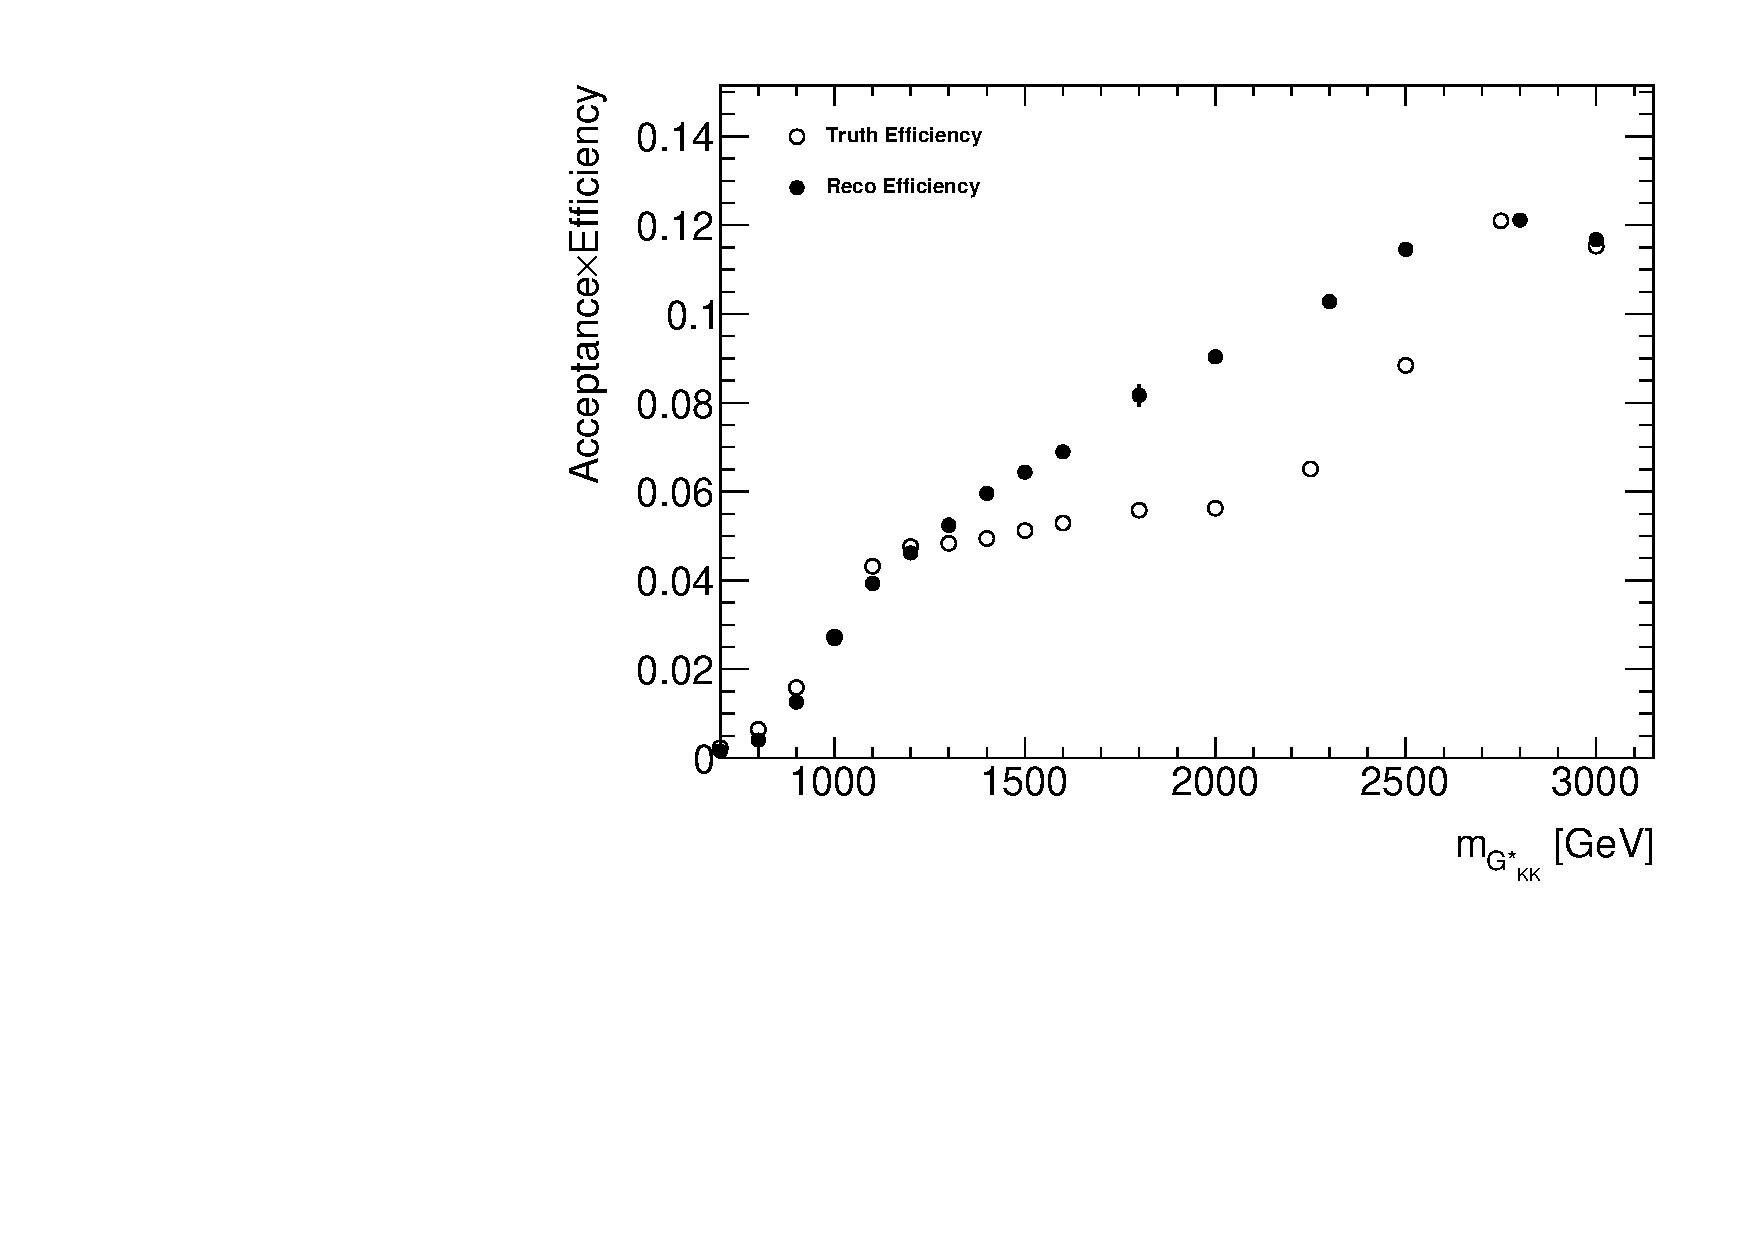
\includegraphics[width=0.3\textwidth, clip]{figures/boosted/Syst_MC/Boosted_2Tag_BulkRSGKKc1TruthVsReco.pdf}\hspace{5mm}}
% \subfloat[]{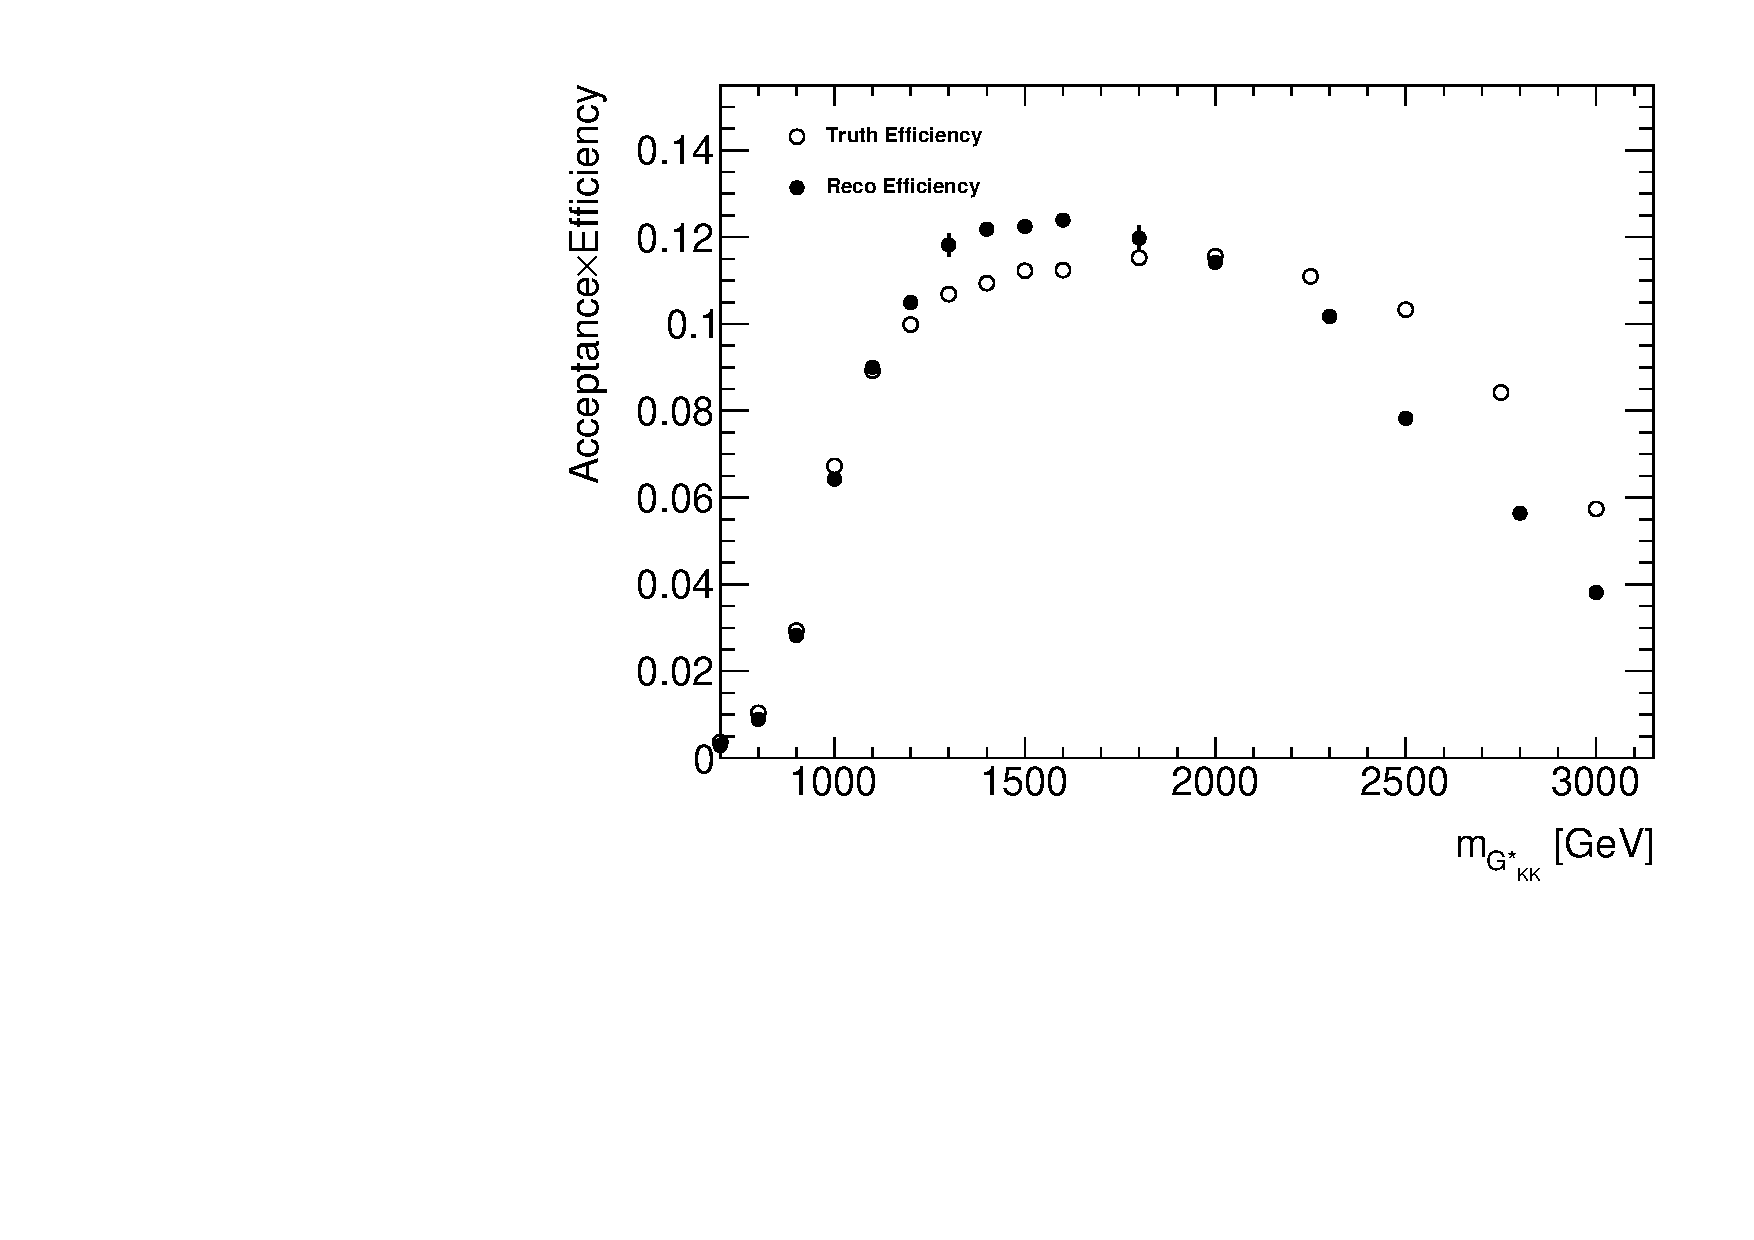
\includegraphics[width=0.3\textwidth, clip]{figures/boosted/Syst_MC/Boosted_3Tag_BulkRSGKKc1TruthVsReco.pdf}\hspace{5mm}}
% \subfloat[]{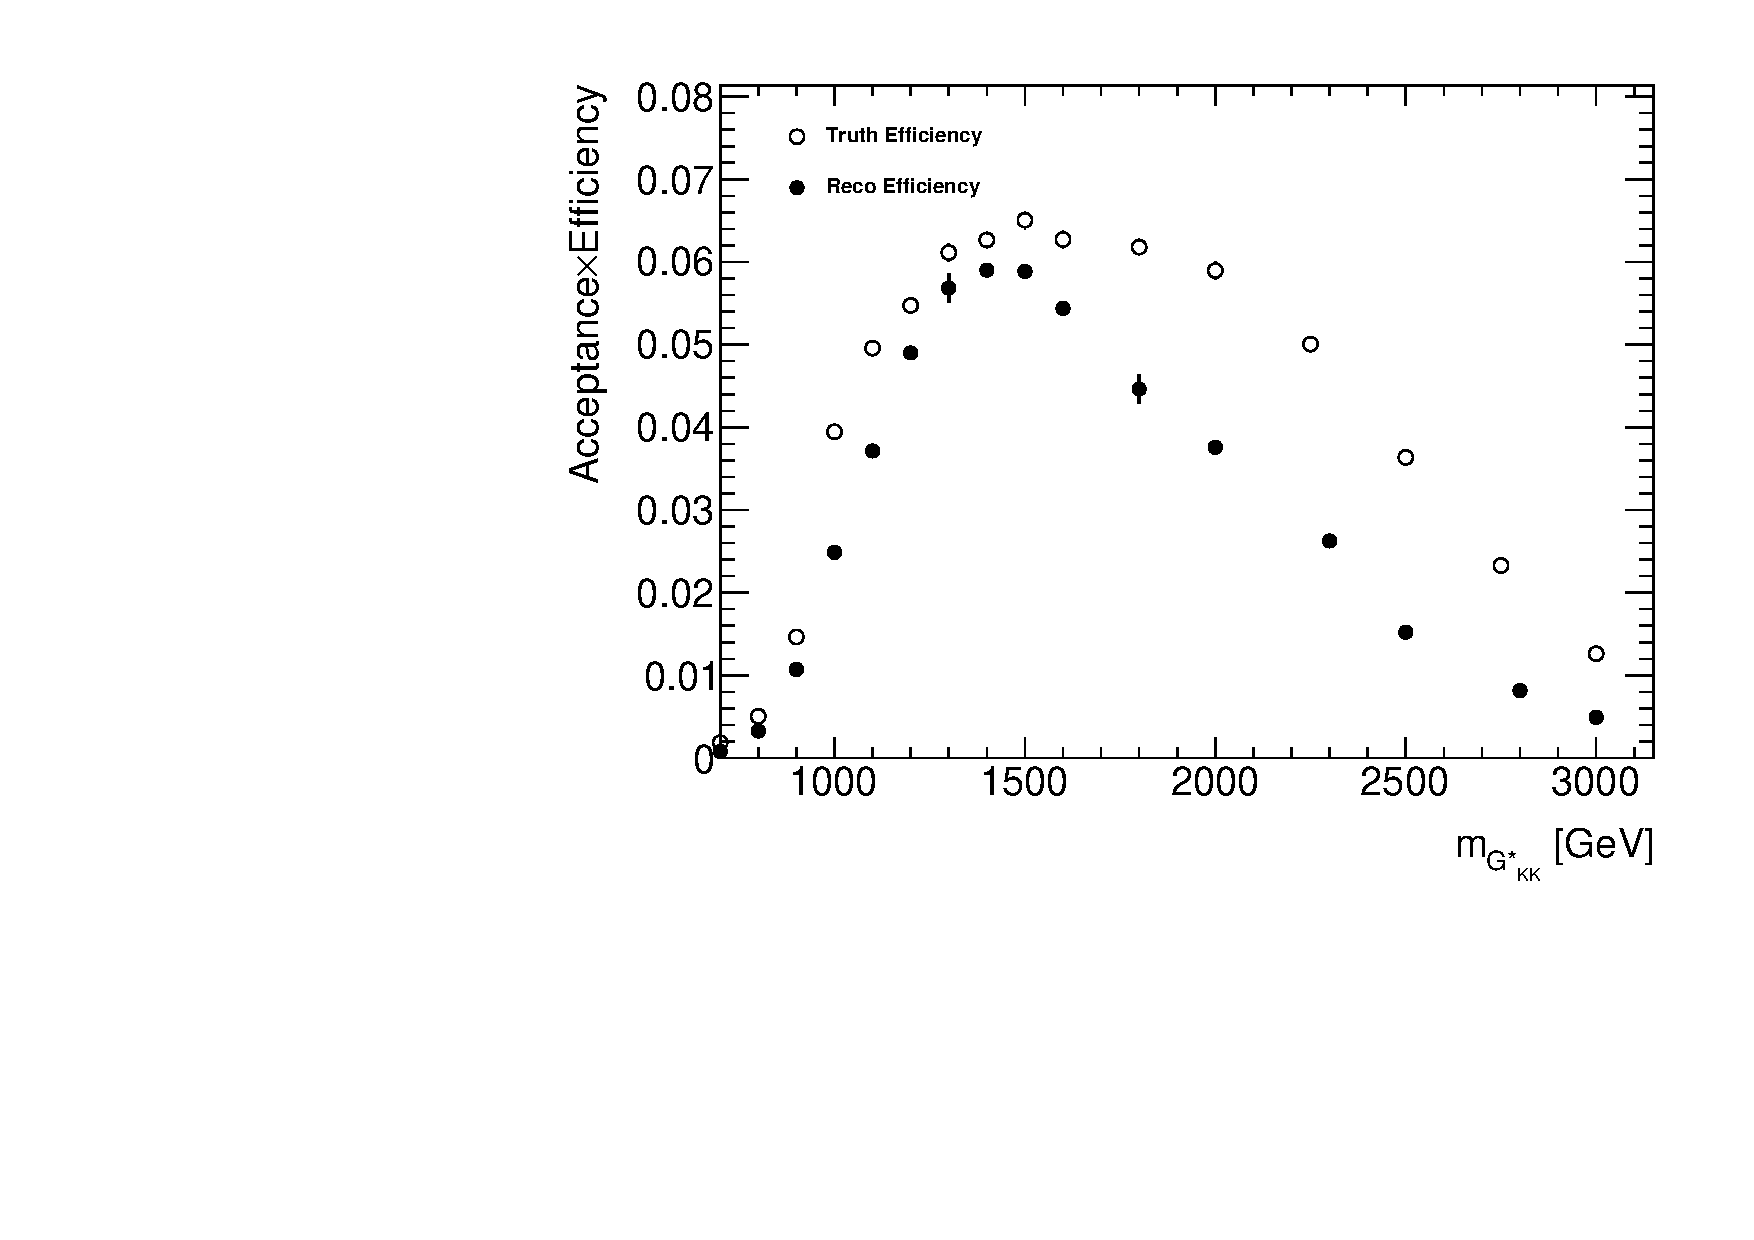
\includegraphics[width=0.3\textwidth, clip]{figures/boosted/Syst_MC/Boosted_4Tag_BulkRSGKKc1TruthVsReco.pdf}\hspace{5mm}}
% \caption{Acceptance times efficiency measured in the particle-level analysis (open circles) and full, reconstruction-level analysis (filled circles) for the graviton in the Bulk-RS model with $c=1$. (a) shows the 2-tag-split selection; (b) shows the 3-tag selection; and (c) shows the 4-tag selection}
% \label{fig:AccxEff_truthVsReco}
% \end{center}
% \end{figure*}

%%\paragraph{}
To evaluate the potential effect of missing higher order terms in the matrix element, the renormalisation and factorisation scales used in the signal generation were varied coherently by factors of $0.5\times$ and $2\times$ for the signals. The effect is shown as function of resonance mass in Figure \ref{fig:scaleVar}.

% \begin{figure*}
% \begin{center}
% \subfloat[2-Tag-Split: bulk RS c=1]{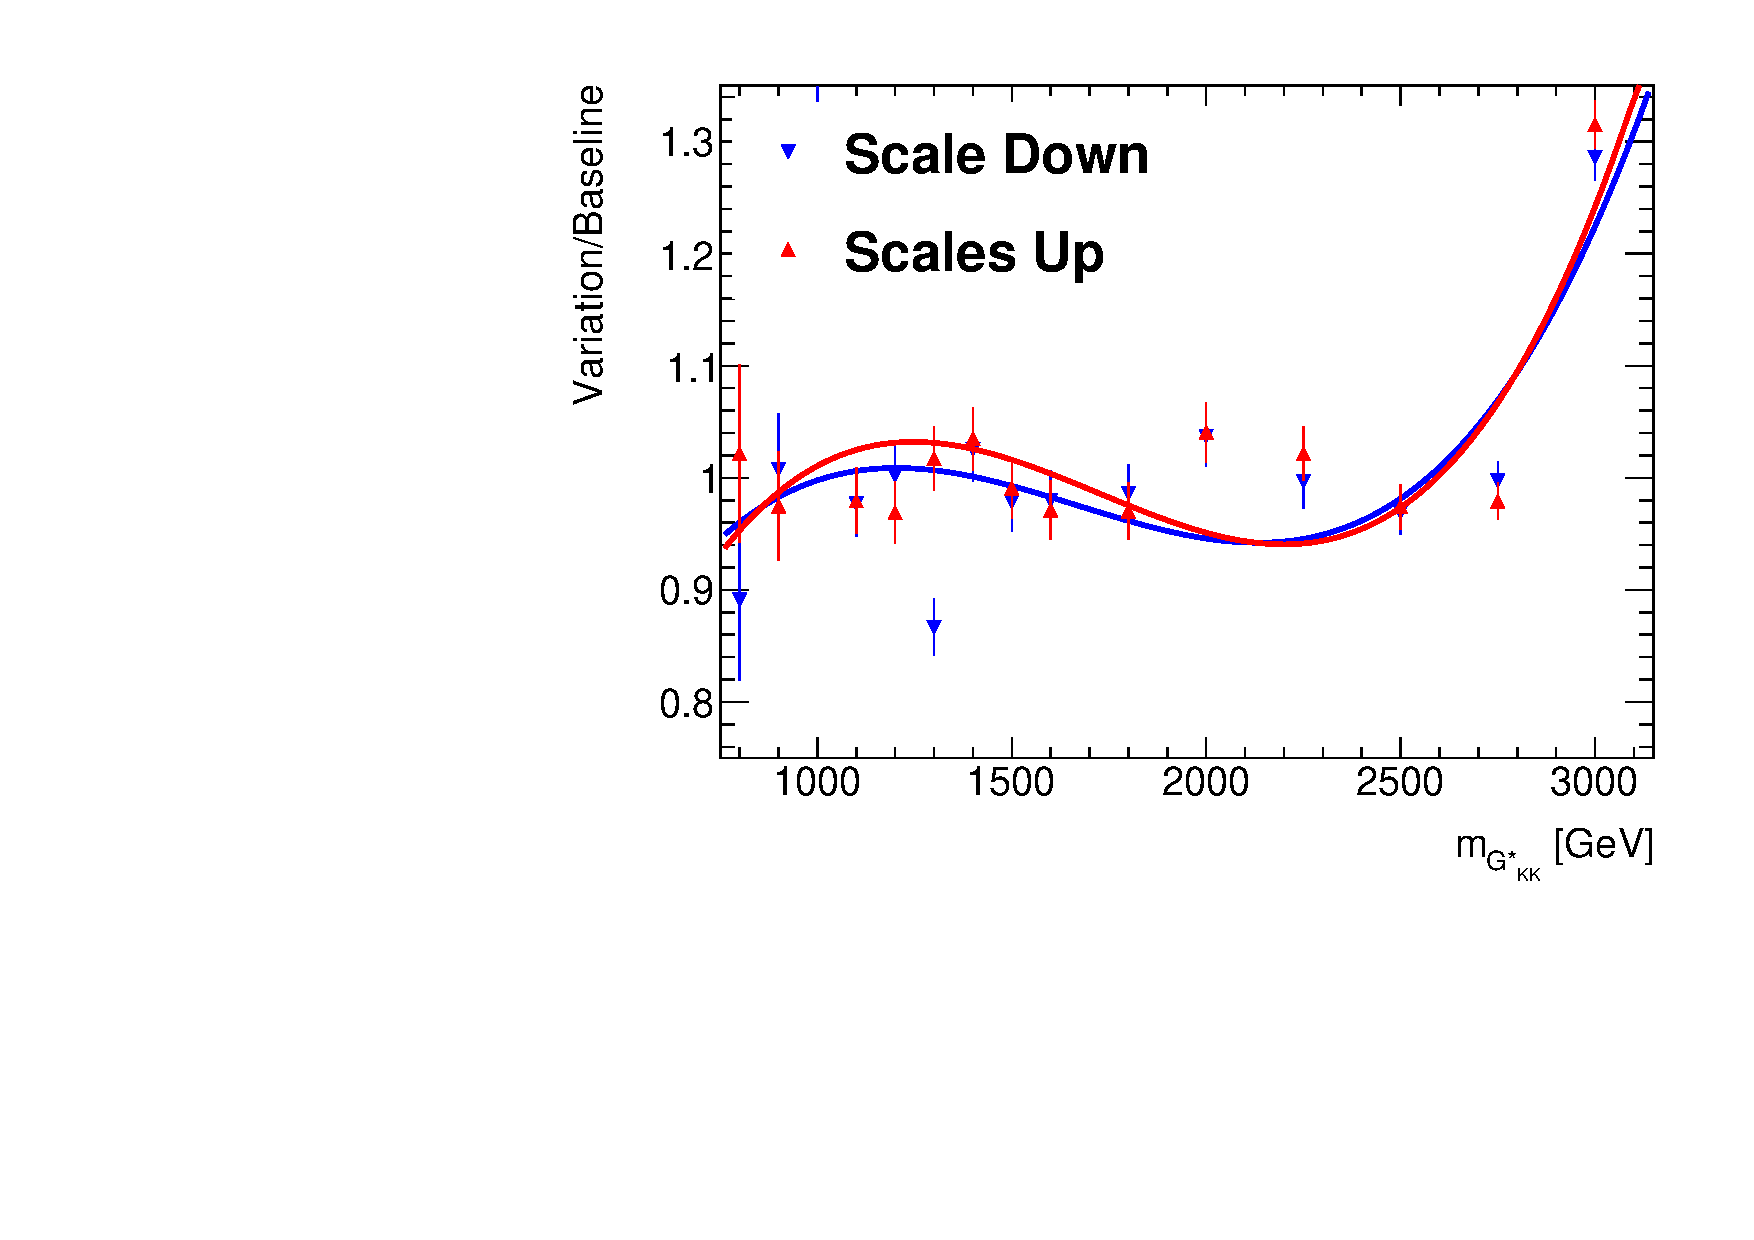
\includegraphics[width=0.3\textwidth, clip]{figures/boosted/Syst_MC/Boosted_2Tag_BulkRSGKKc1_Scale_ratio.pdf}\hspace{5mm}}
% \subfloat[2-Tag-Split: bulk RS c=2]{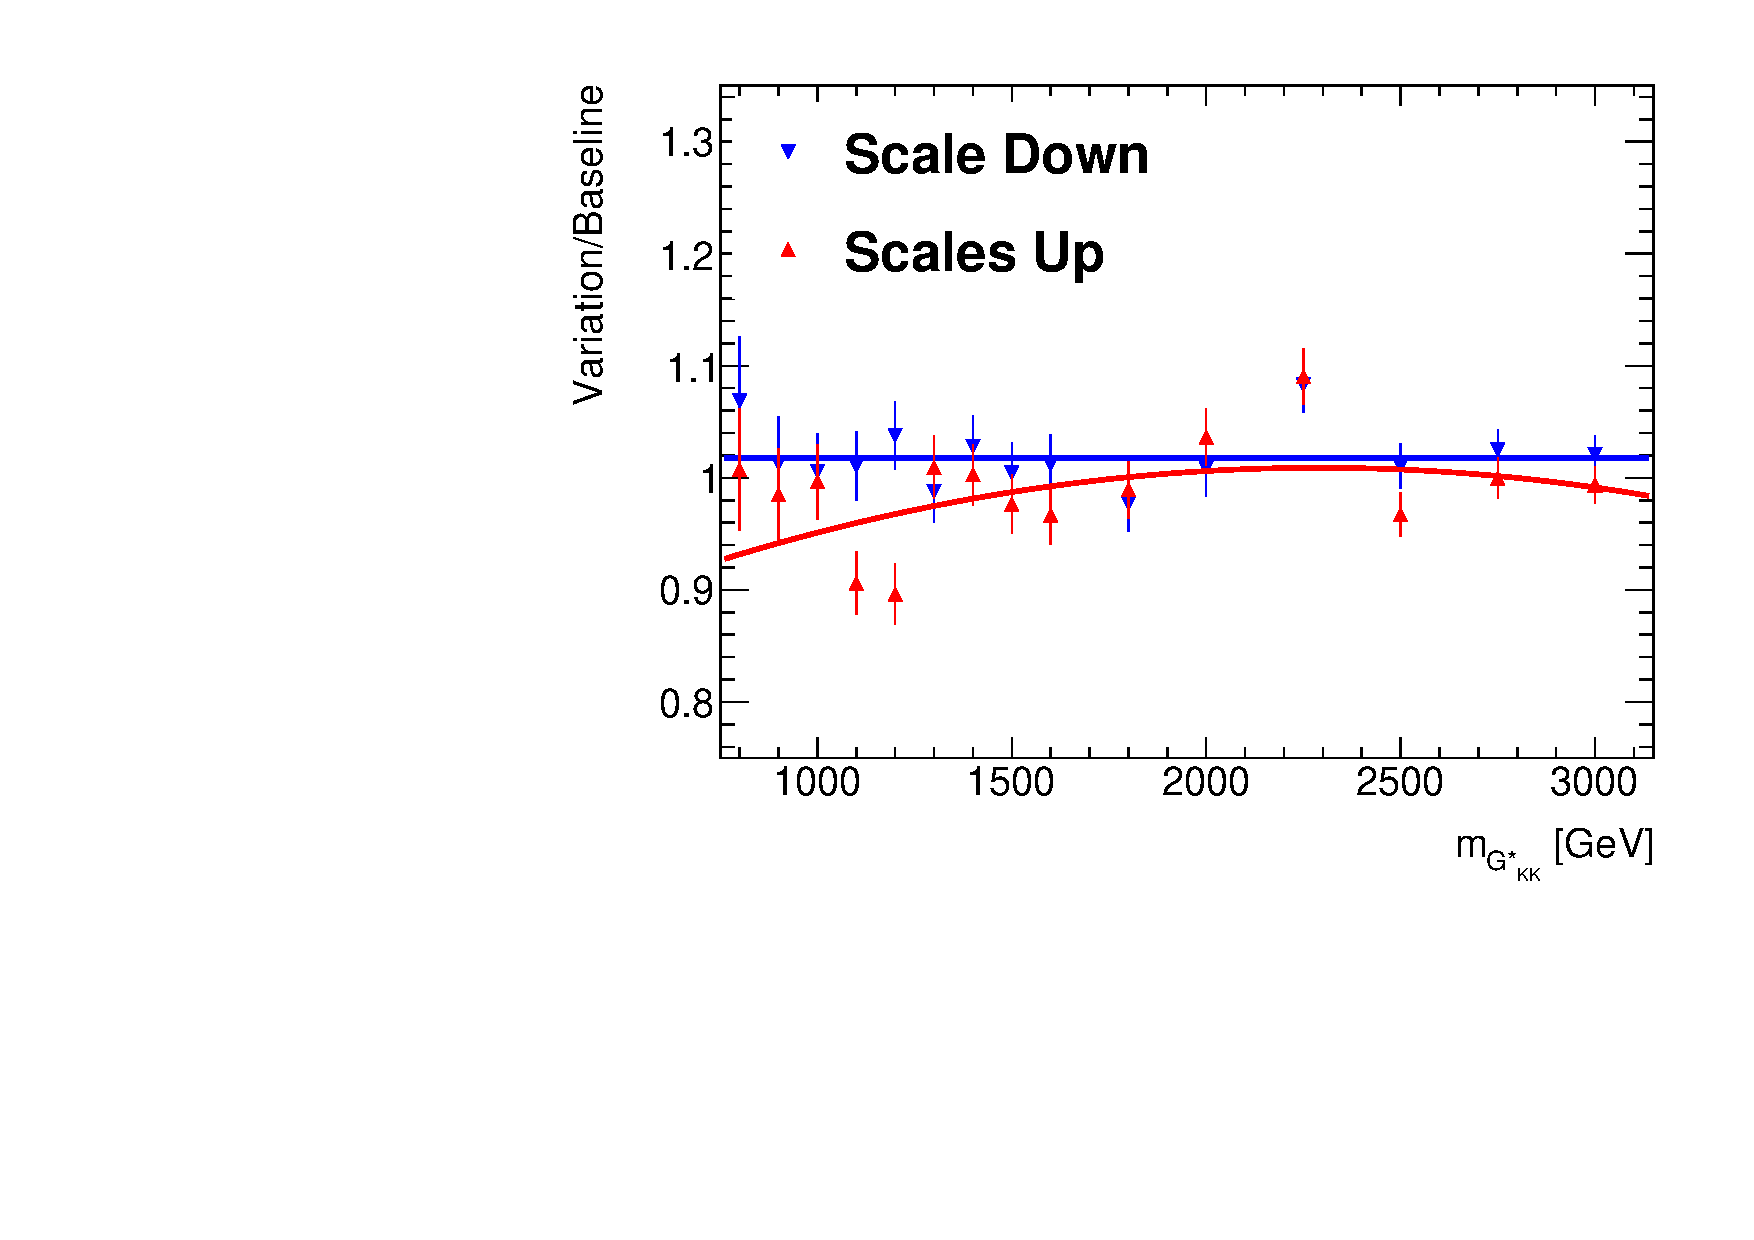
\includegraphics[width=0.3\textwidth, clip]{figures/boosted/Syst_MC/Boosted_2Tag_BulkRSGKKc2_Scale_ratio.pdf}\hspace{5mm}}
% \subfloat[2-Tag-Split: scalar]{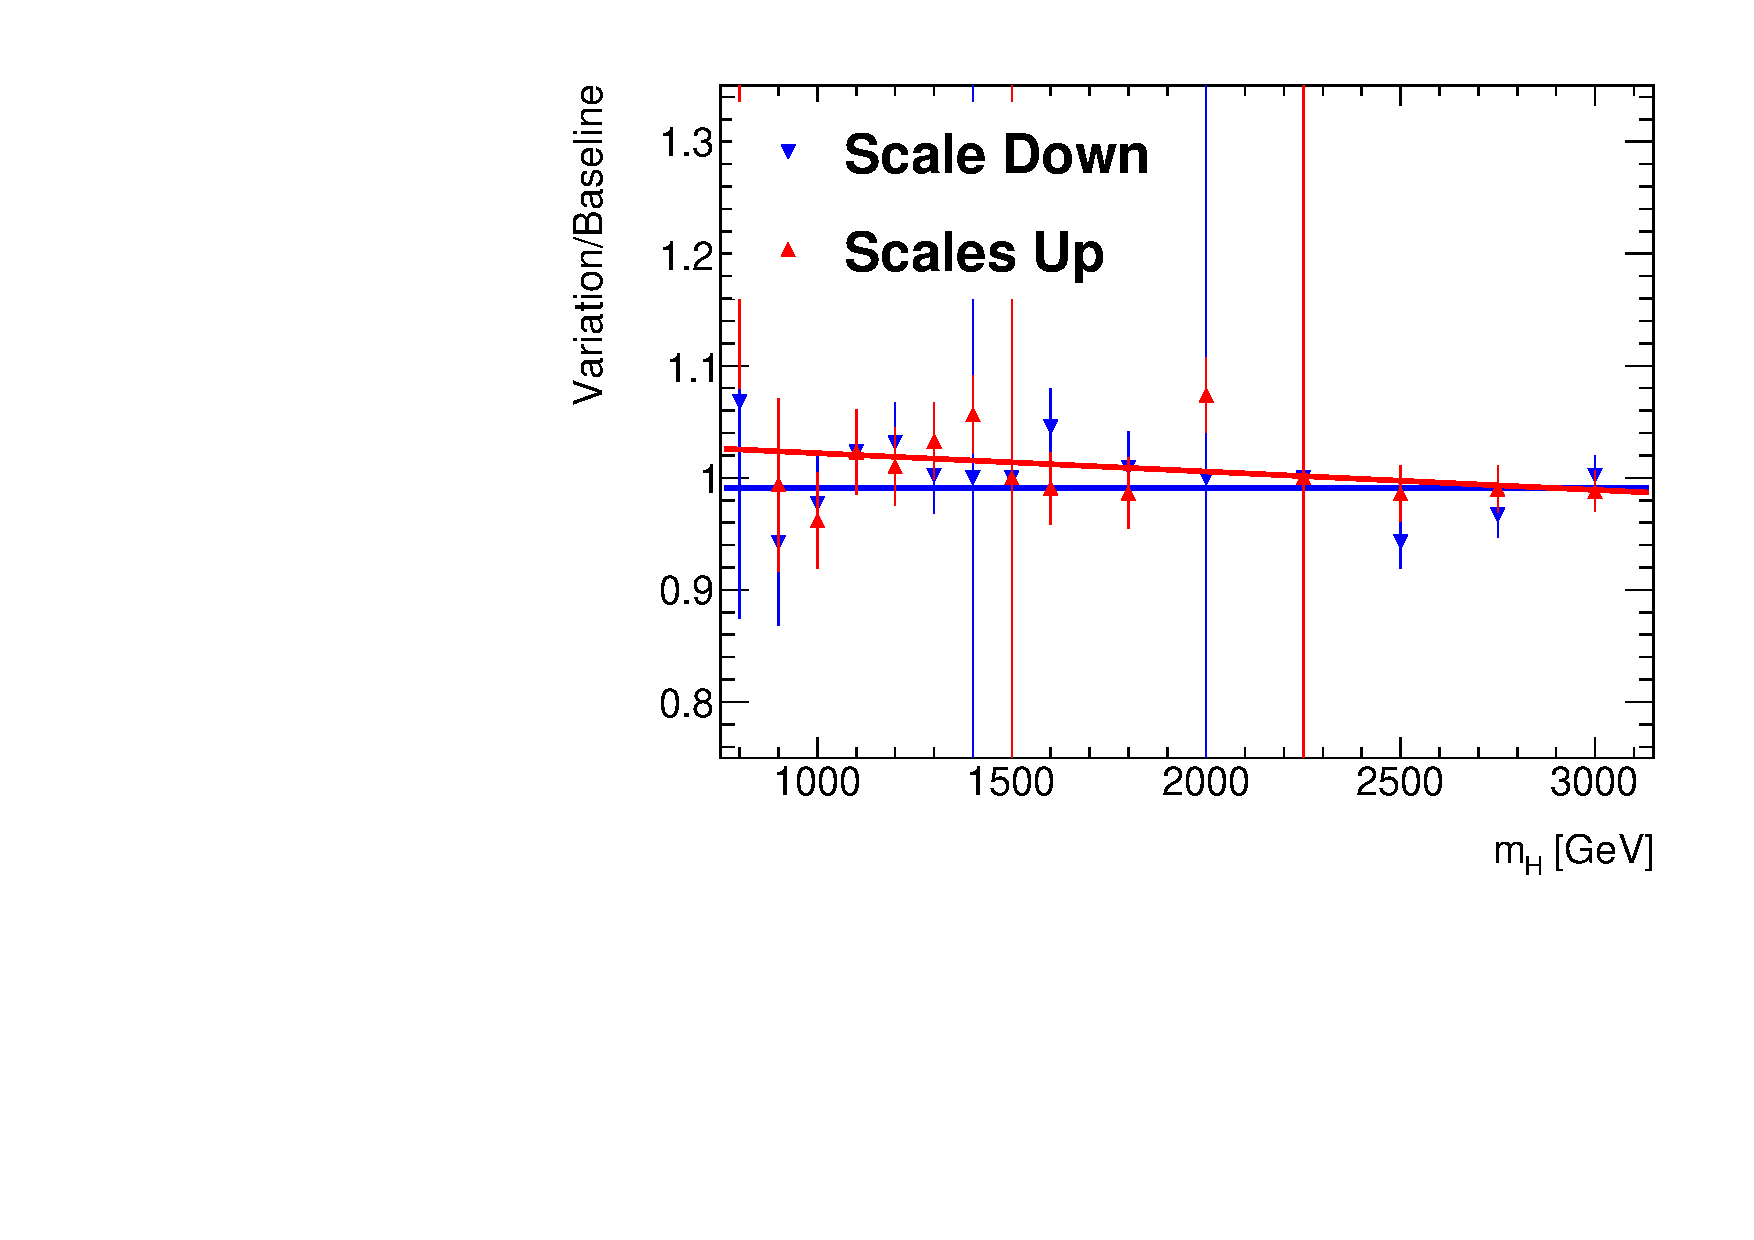
\includegraphics[width=0.3\textwidth, clip]{figures/boosted/Syst_MC/Boosted_2Tag_Scalar_Scale_ratio.pdf}\hspace{5mm}}\\
% \subfloat[3-Tag: bulk RS c=1]{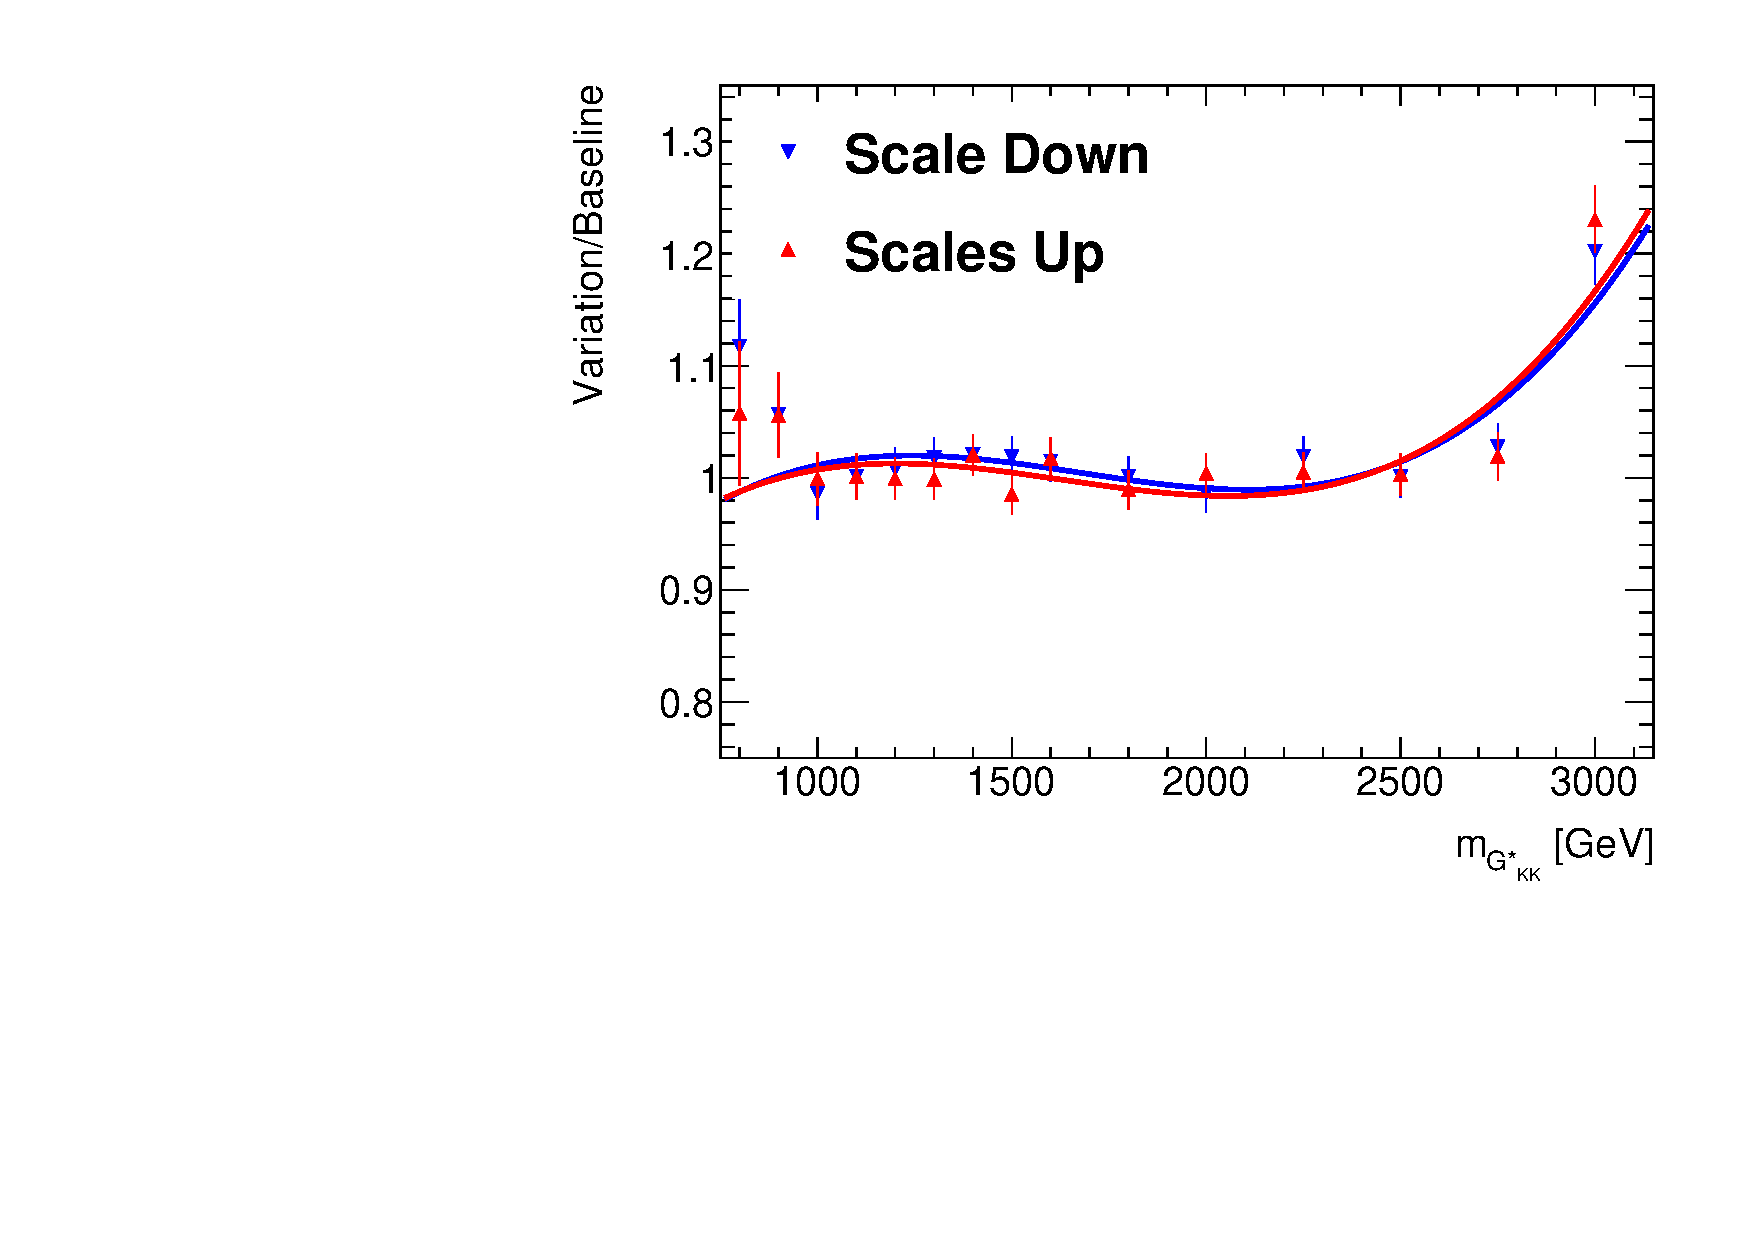
\includegraphics[width=0.3\textwidth, clip]{figures/boosted/Syst_MC/Boosted_3Tag_BulkRSGKKc1_Scale_ratio.pdf}\hspace{5mm}}
% \subfloat[3-Tag: bulk RS c=2]{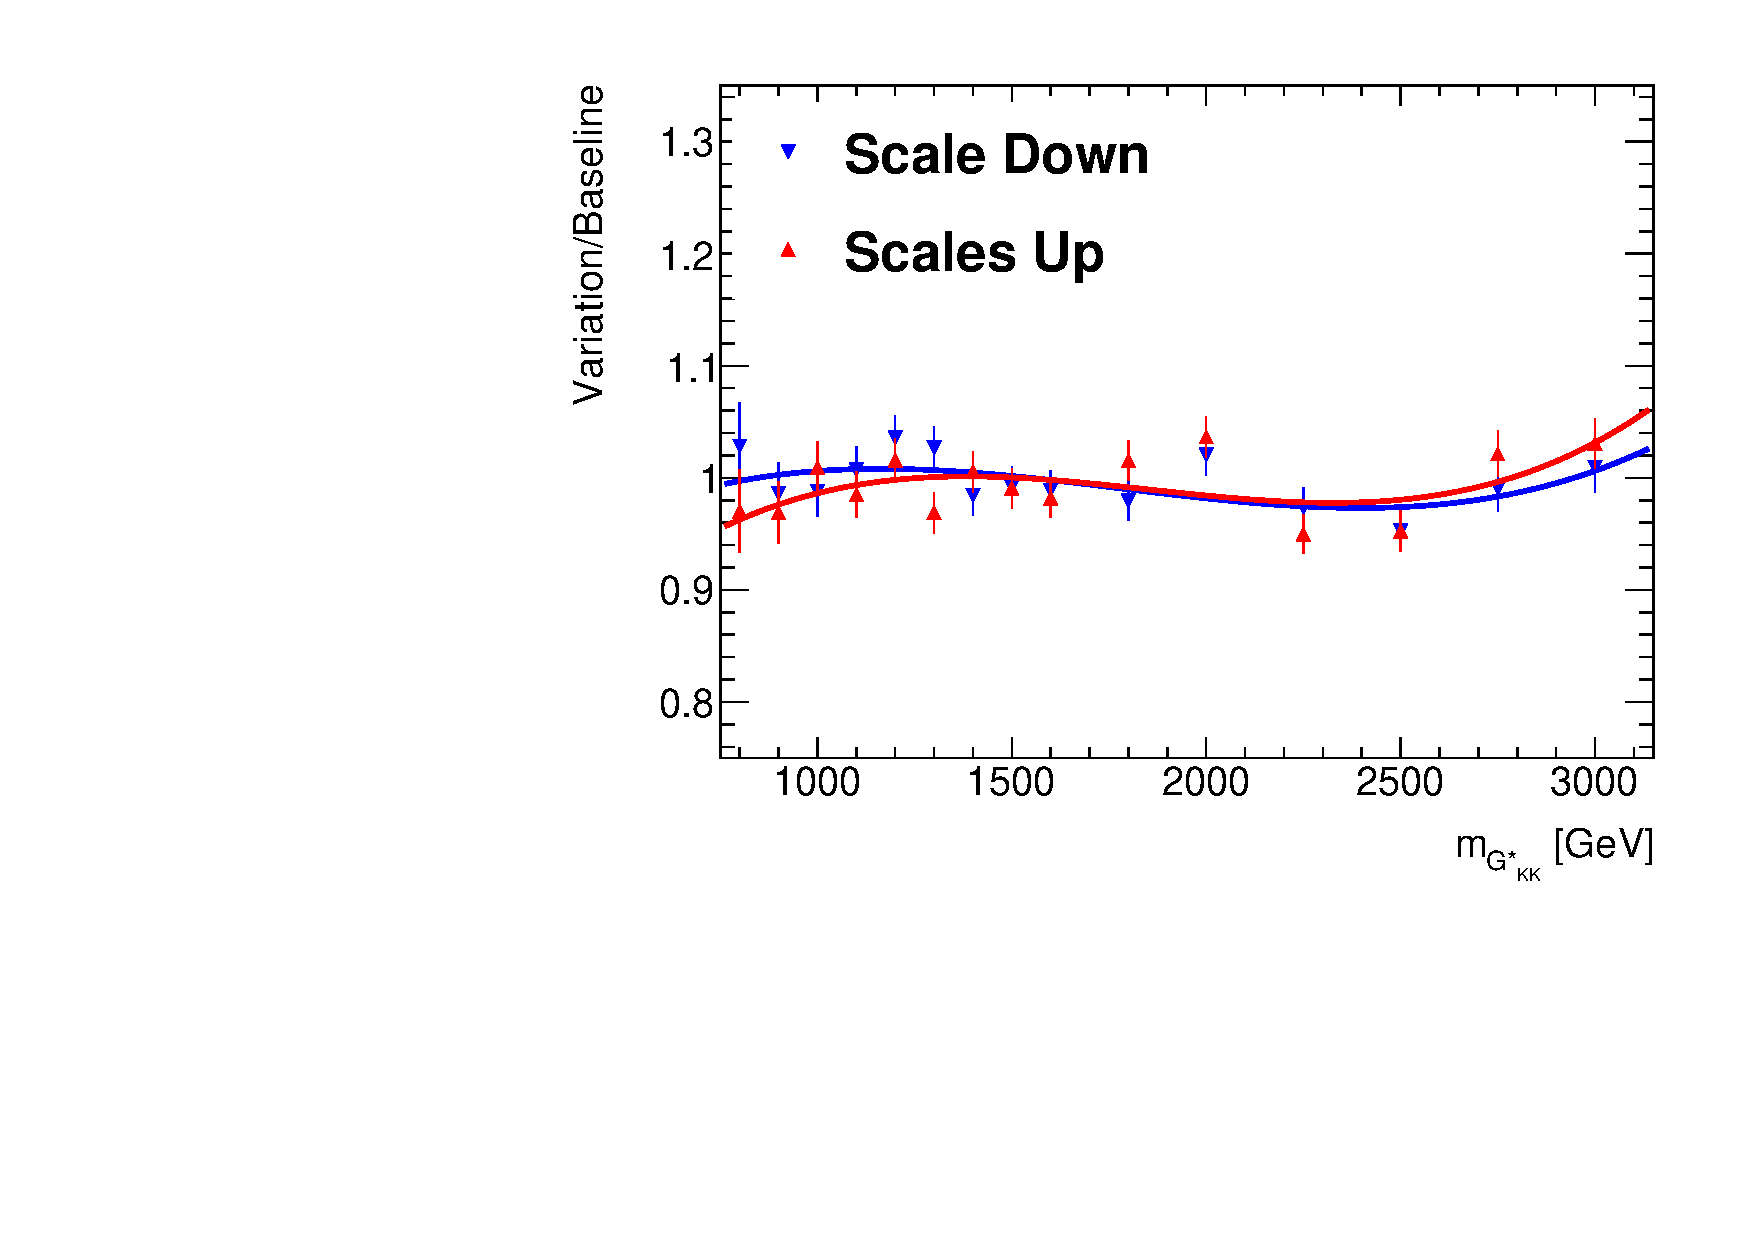
\includegraphics[width=0.3\textwidth, clip]{figures/boosted/Syst_MC/Boosted_3Tag_BulkRSGKKc2_Scale_ratio.pdf}\hspace{5mm}}
% \subfloat[3-Tag: scalar]{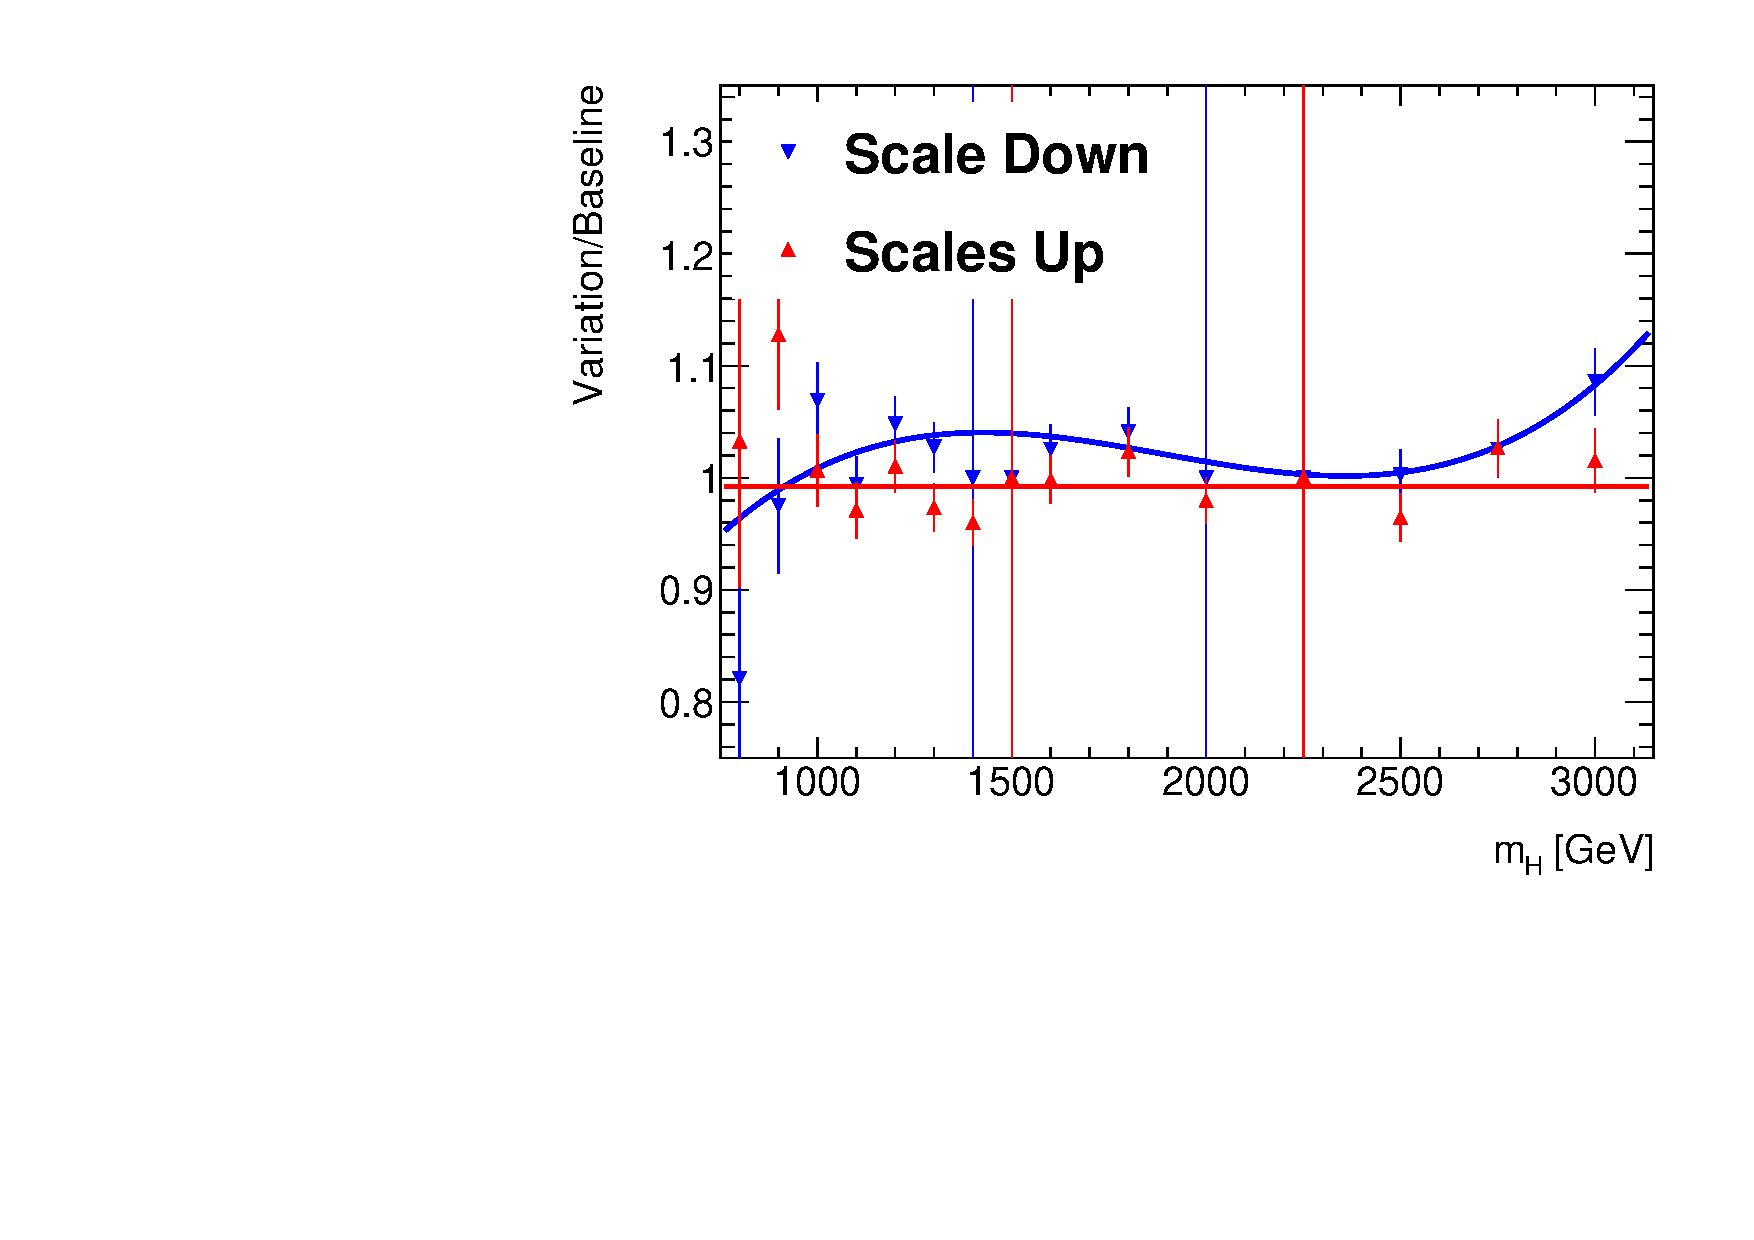
\includegraphics[width=0.3\textwidth, clip]{figures/boosted/Syst_MC/Boosted_3Tag_Scalar_Scale_ratio.pdf}\hspace{5mm}}\\
% \subfloat[4-Tag: bulk RS c=1]{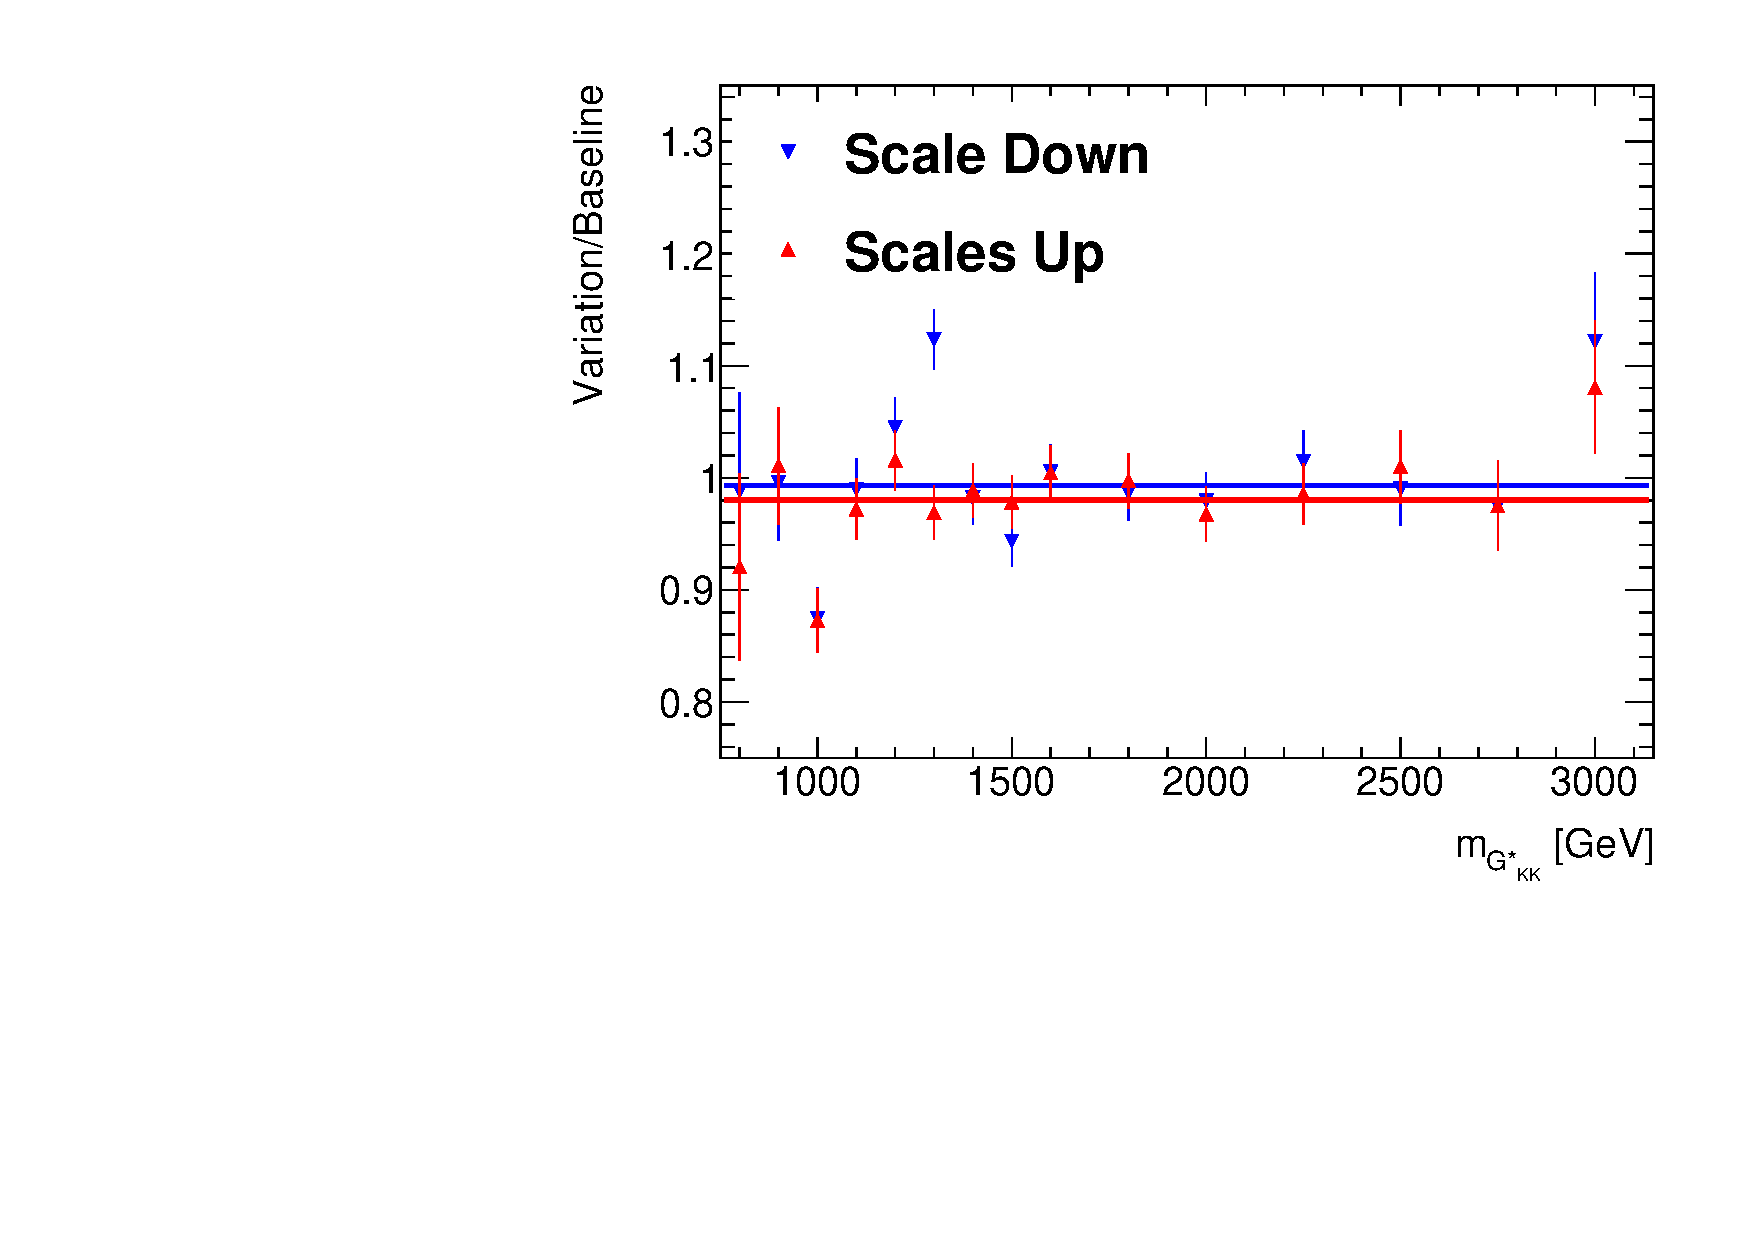
\includegraphics[width=0.3\textwidth, clip]{figures/boosted/Syst_MC/Boosted_4Tag_BulkRSGKKc1_Scale_ratio.pdf}\hspace{5mm}}
% \subfloat[4-Tag: bulk RS c=2]{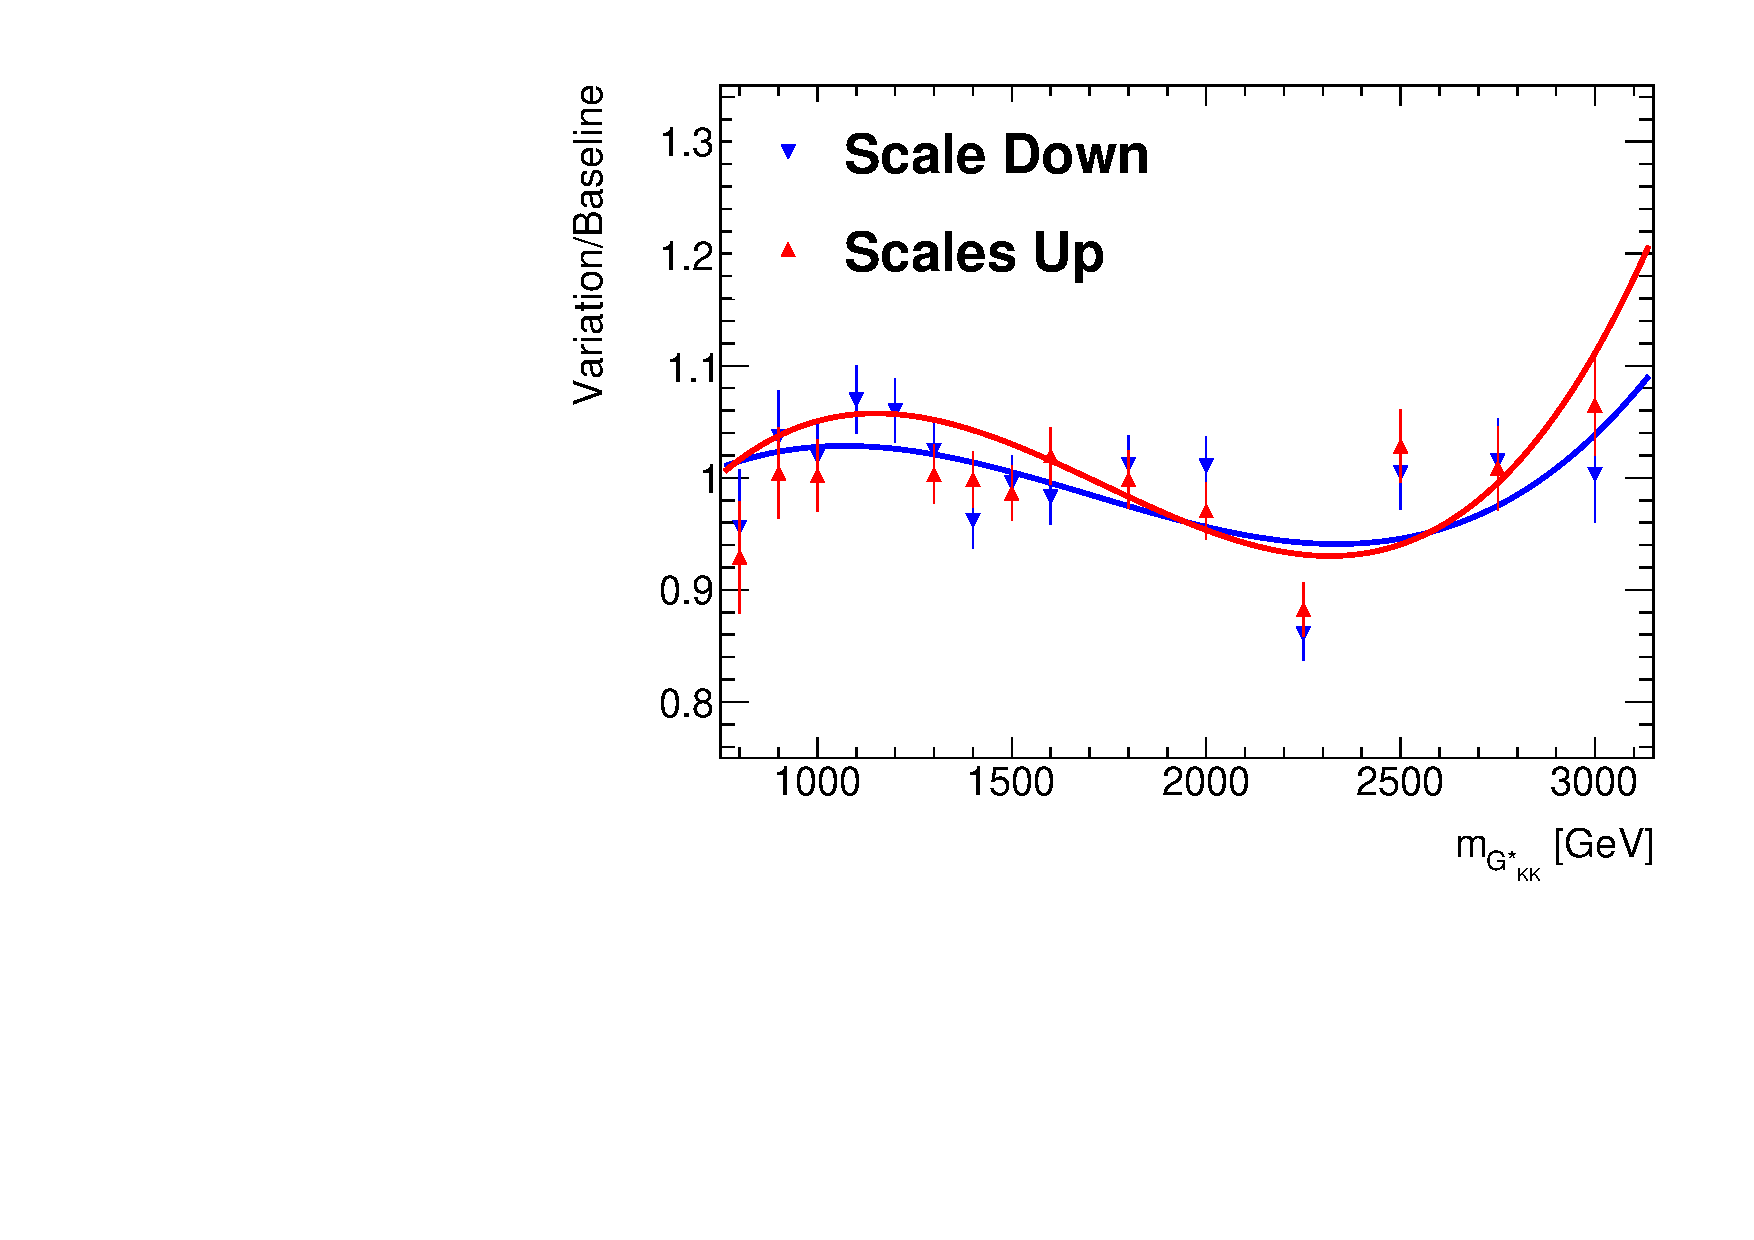
\includegraphics[width=0.3\textwidth, clip]{figures/boosted/Syst_MC/Boosted_4Tag_BulkRSGKKc2_Scale_ratio.pdf}\hspace{5mm}}
% \subfloat[4-Tag: scalar]{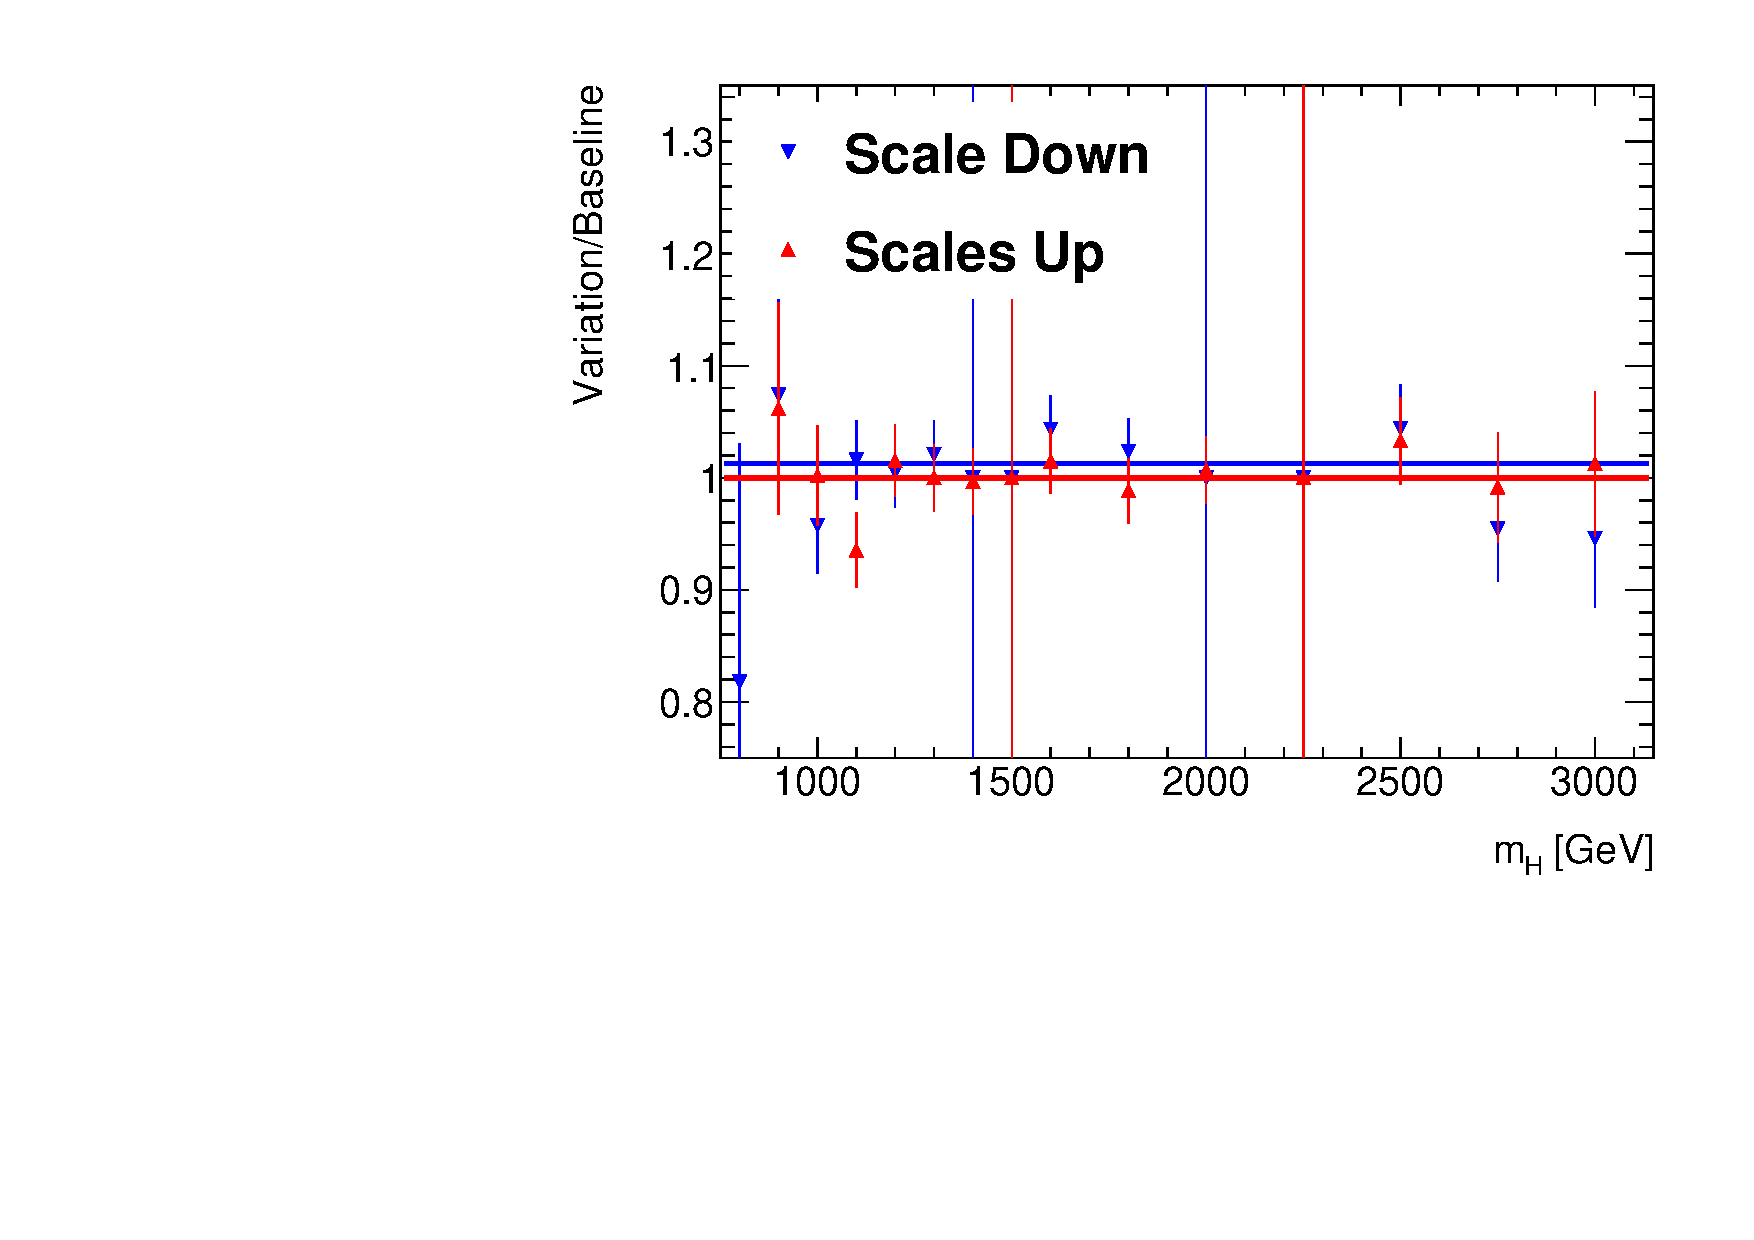
\includegraphics[width=0.3\textwidth, clip]{figures/boosted/Syst_MC/Boosted_4Tag_Scalar_Scale_ratio.pdf}\hspace{5mm}}
% \caption{Ratio of acceptance times efficiency measured in the scale-varied samples over the baseline sample. The upward-pointing triangles correspond to doubling both the renormalisation and factorisation scales, while the downward-pointing triangles correspond to halving them. The polynomial fits shown as solid lines are used to assign the corresponding systematic variation in the final statistical analysis.}
% \label{fig:scaleVar}
% \end{center}
% \end{figure*}

%\paragraph{}
Uncertainties due to modelling of the parton shower and the underlying event (including multi-parton interactions) are evaluated by switching the MC generator used. For the Bulk RS graviton samples, this means switching from Pythia 8 to Herwig++, while for the scalar and non-resonant it is Herwig++ to Pythia 8. Figure \ref{fig:showerVar} shows the impact of these variations on the signal acceptance.

% \begin{figure*}
% \begin{center}
% \subfloat[2-Tag-Split: bulk RS c=1]{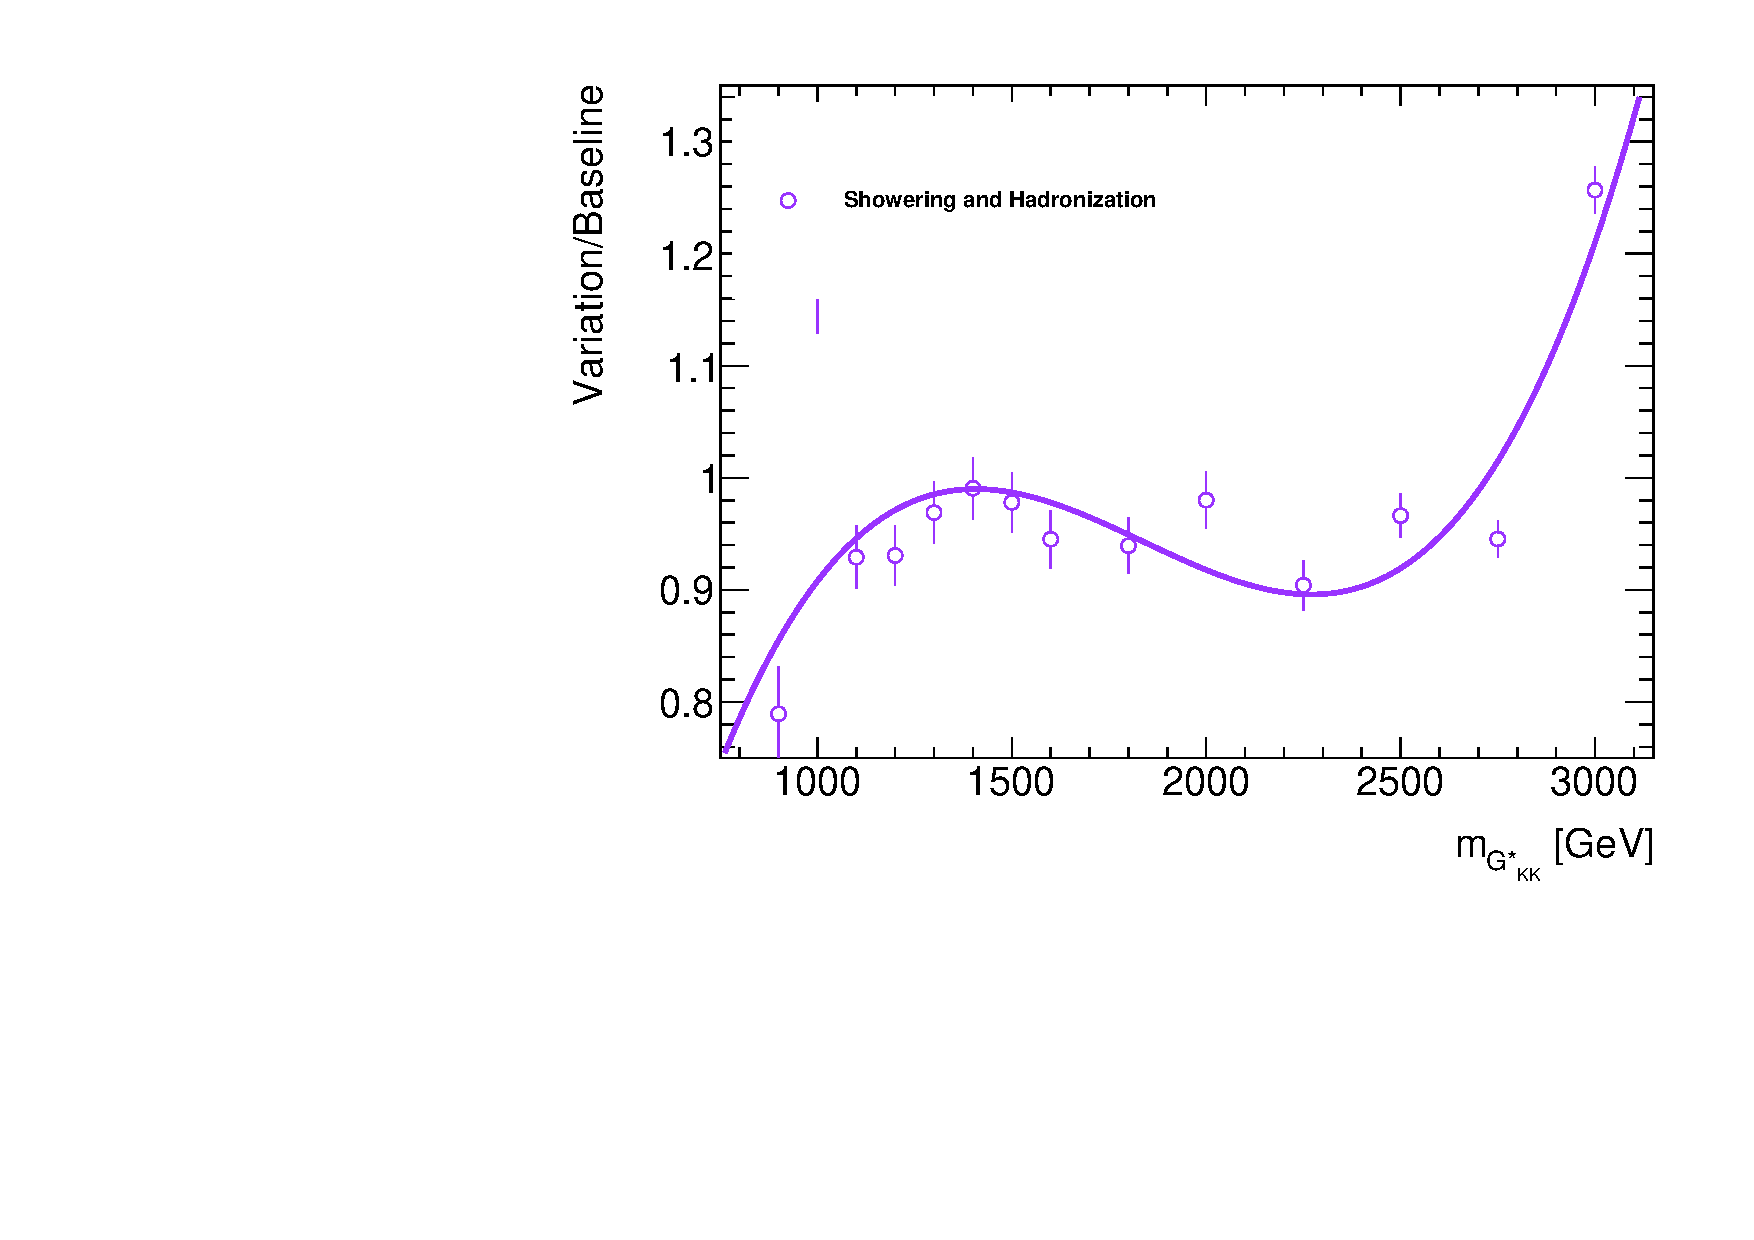
\includegraphics[width=0.3\textwidth, clip]{figures/boosted/Syst_MC/Boosted_2Tag_BulkRSGKKc1_Shower_ratio.pdf}\hspace{5mm}}
% \subfloat[2-Tag-Split: bulk RS c=2]{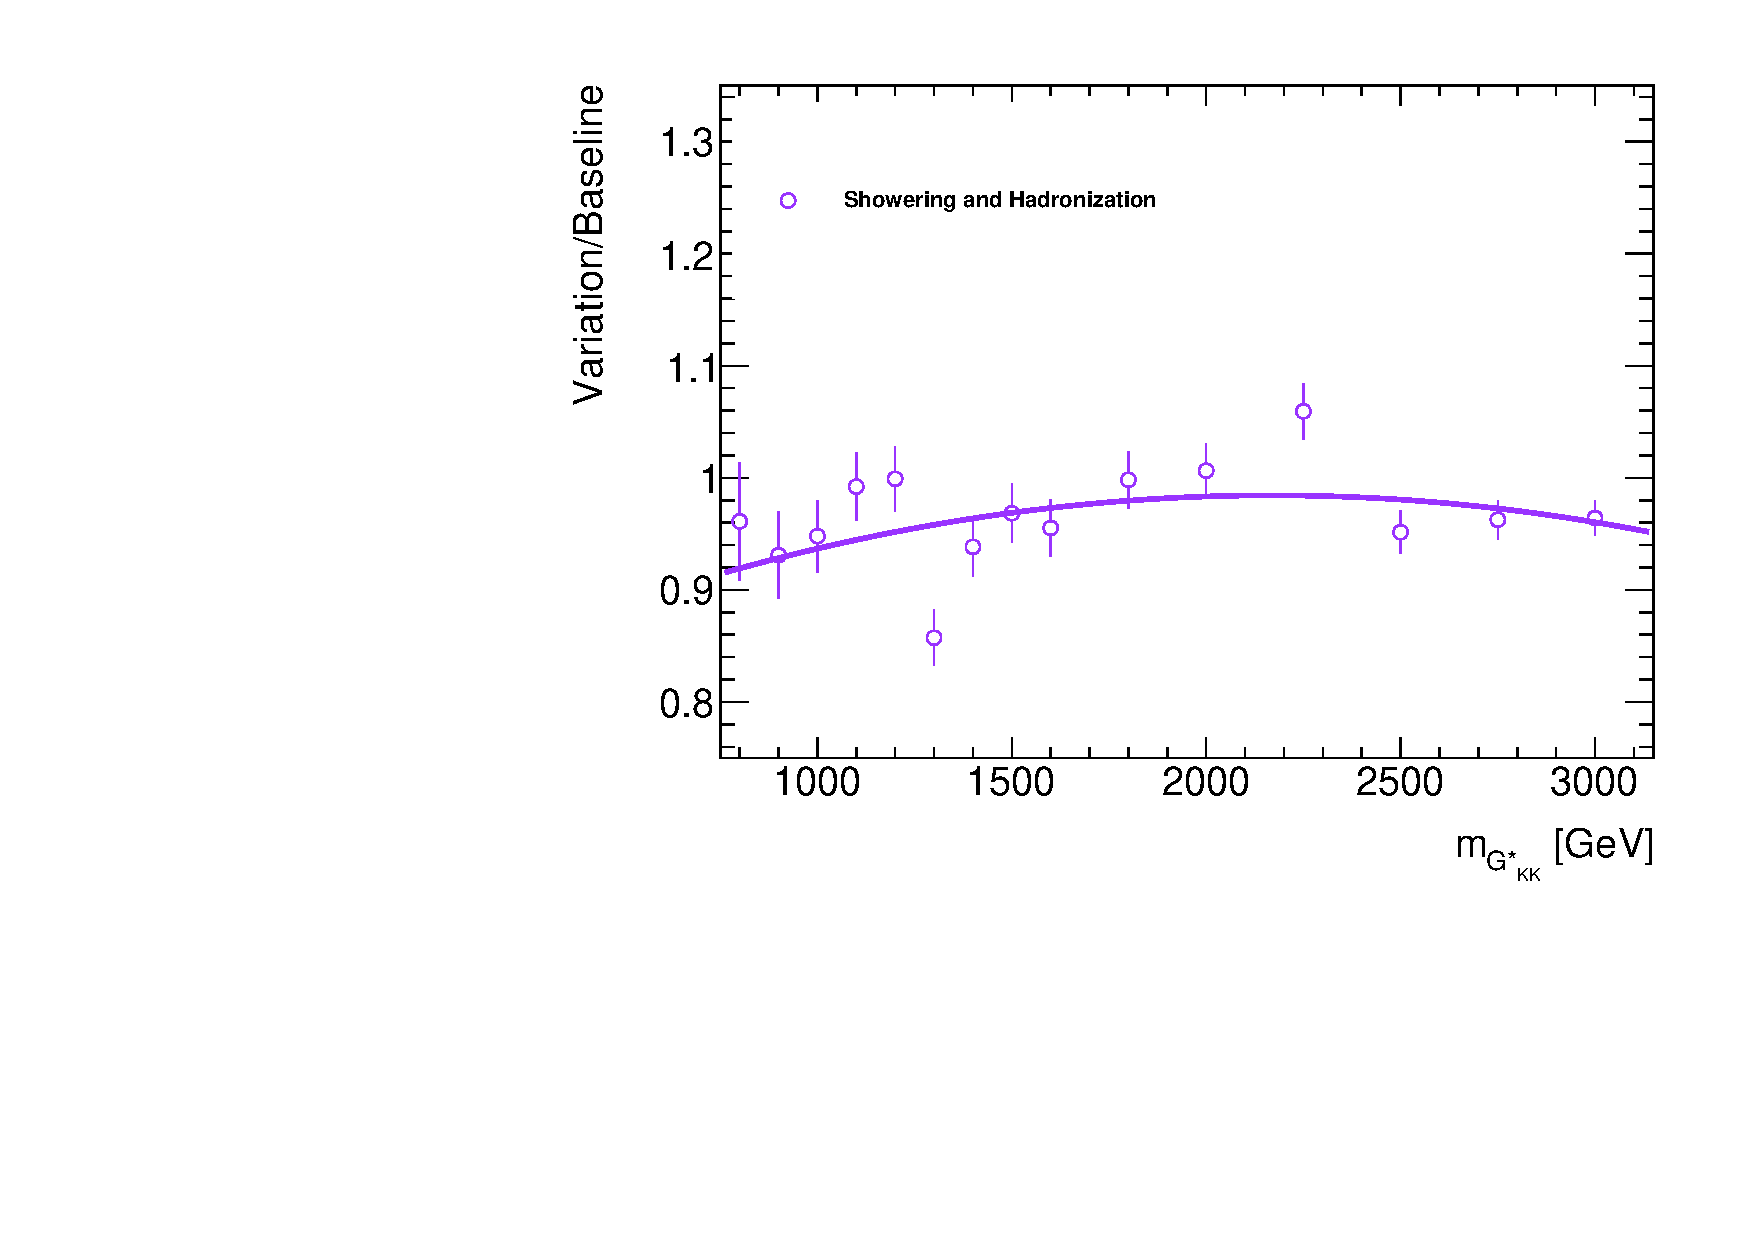
\includegraphics[width=0.3\textwidth, clip]{figures/boosted/Syst_MC/Boosted_2Tag_BulkRSGKKc2_Shower_ratio.pdf}\hspace{5mm}}
% \subfloat[2-Tag-Split: scalar]{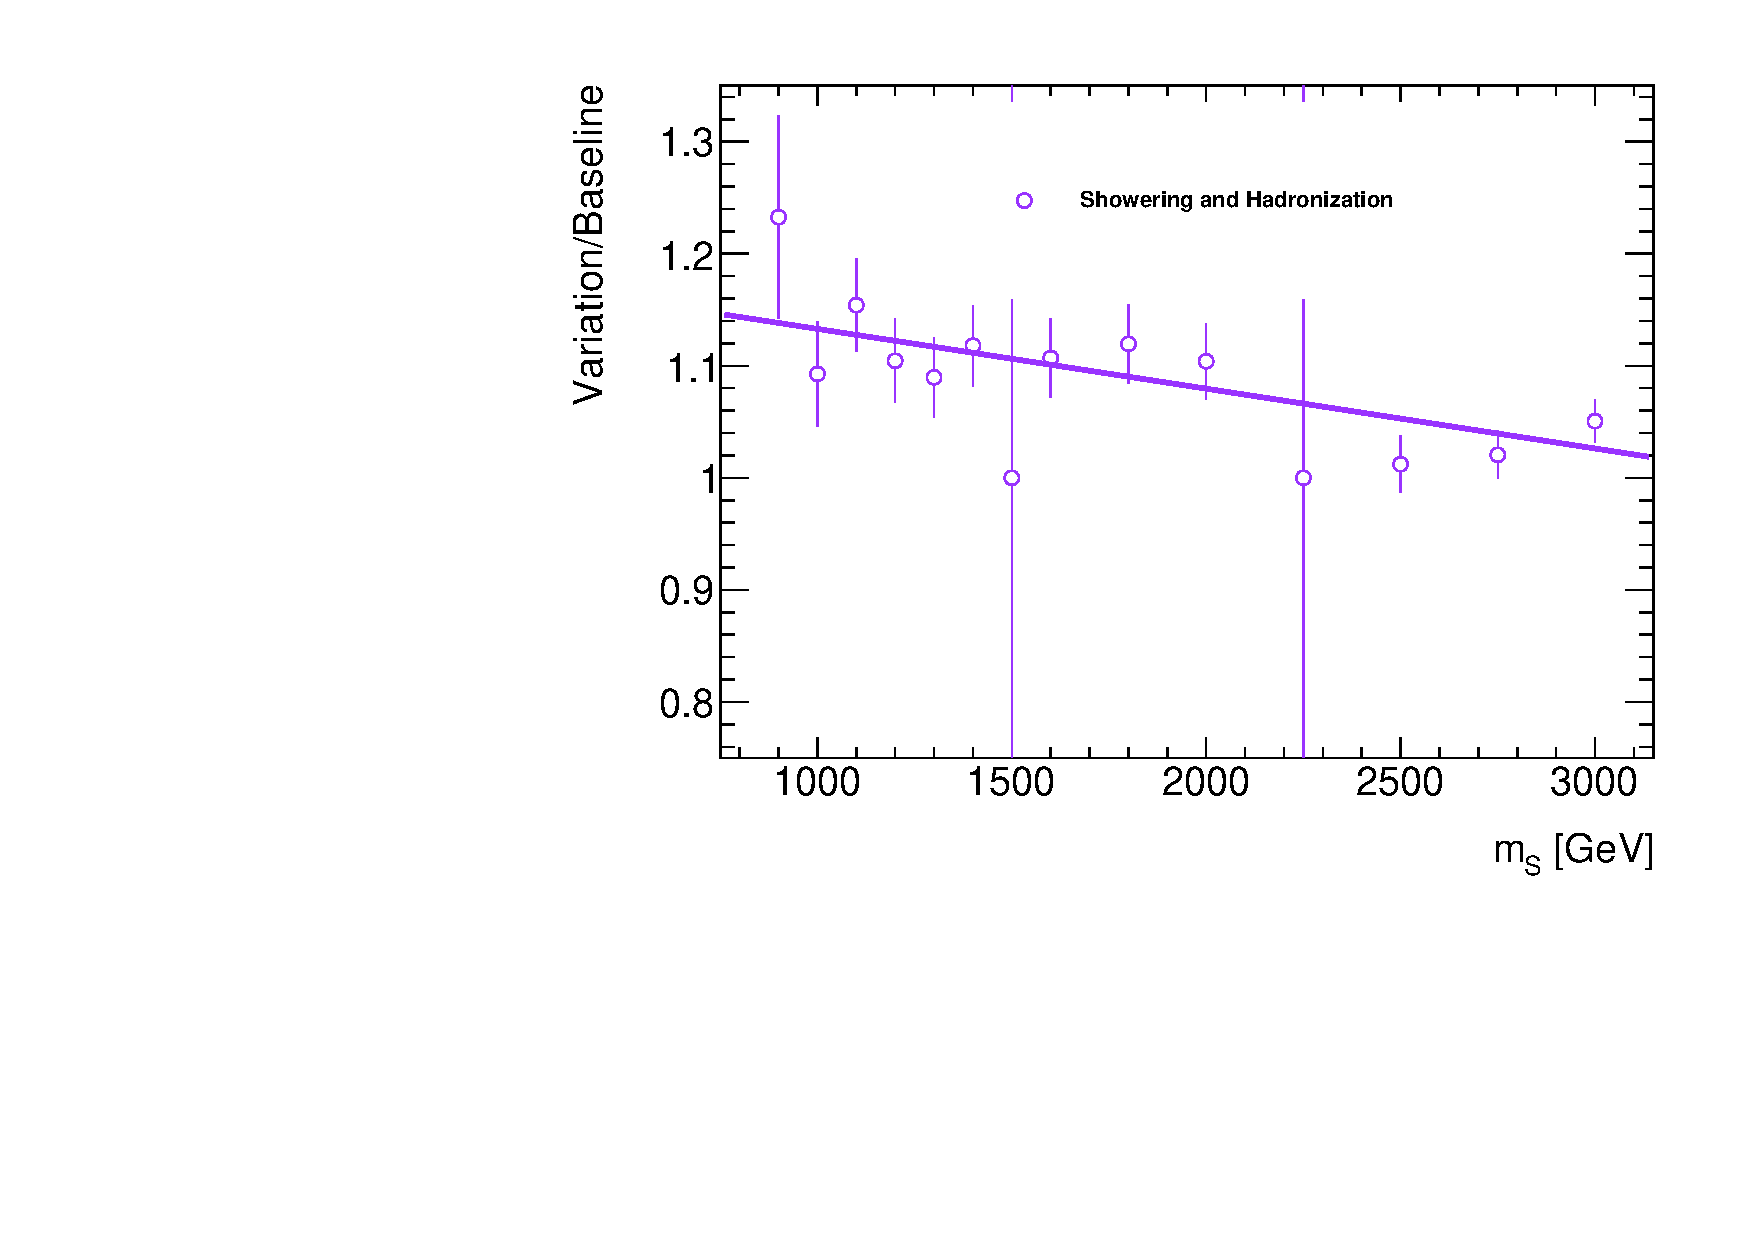
\includegraphics[width=0.3\textwidth, clip]{figures/boosted/Syst_MC/Boosted_2Tag_Scalar_Shower_ratio.pdf}\hspace{5mm}}\\
% \subfloat[3-Tag: bulk RS c=1]{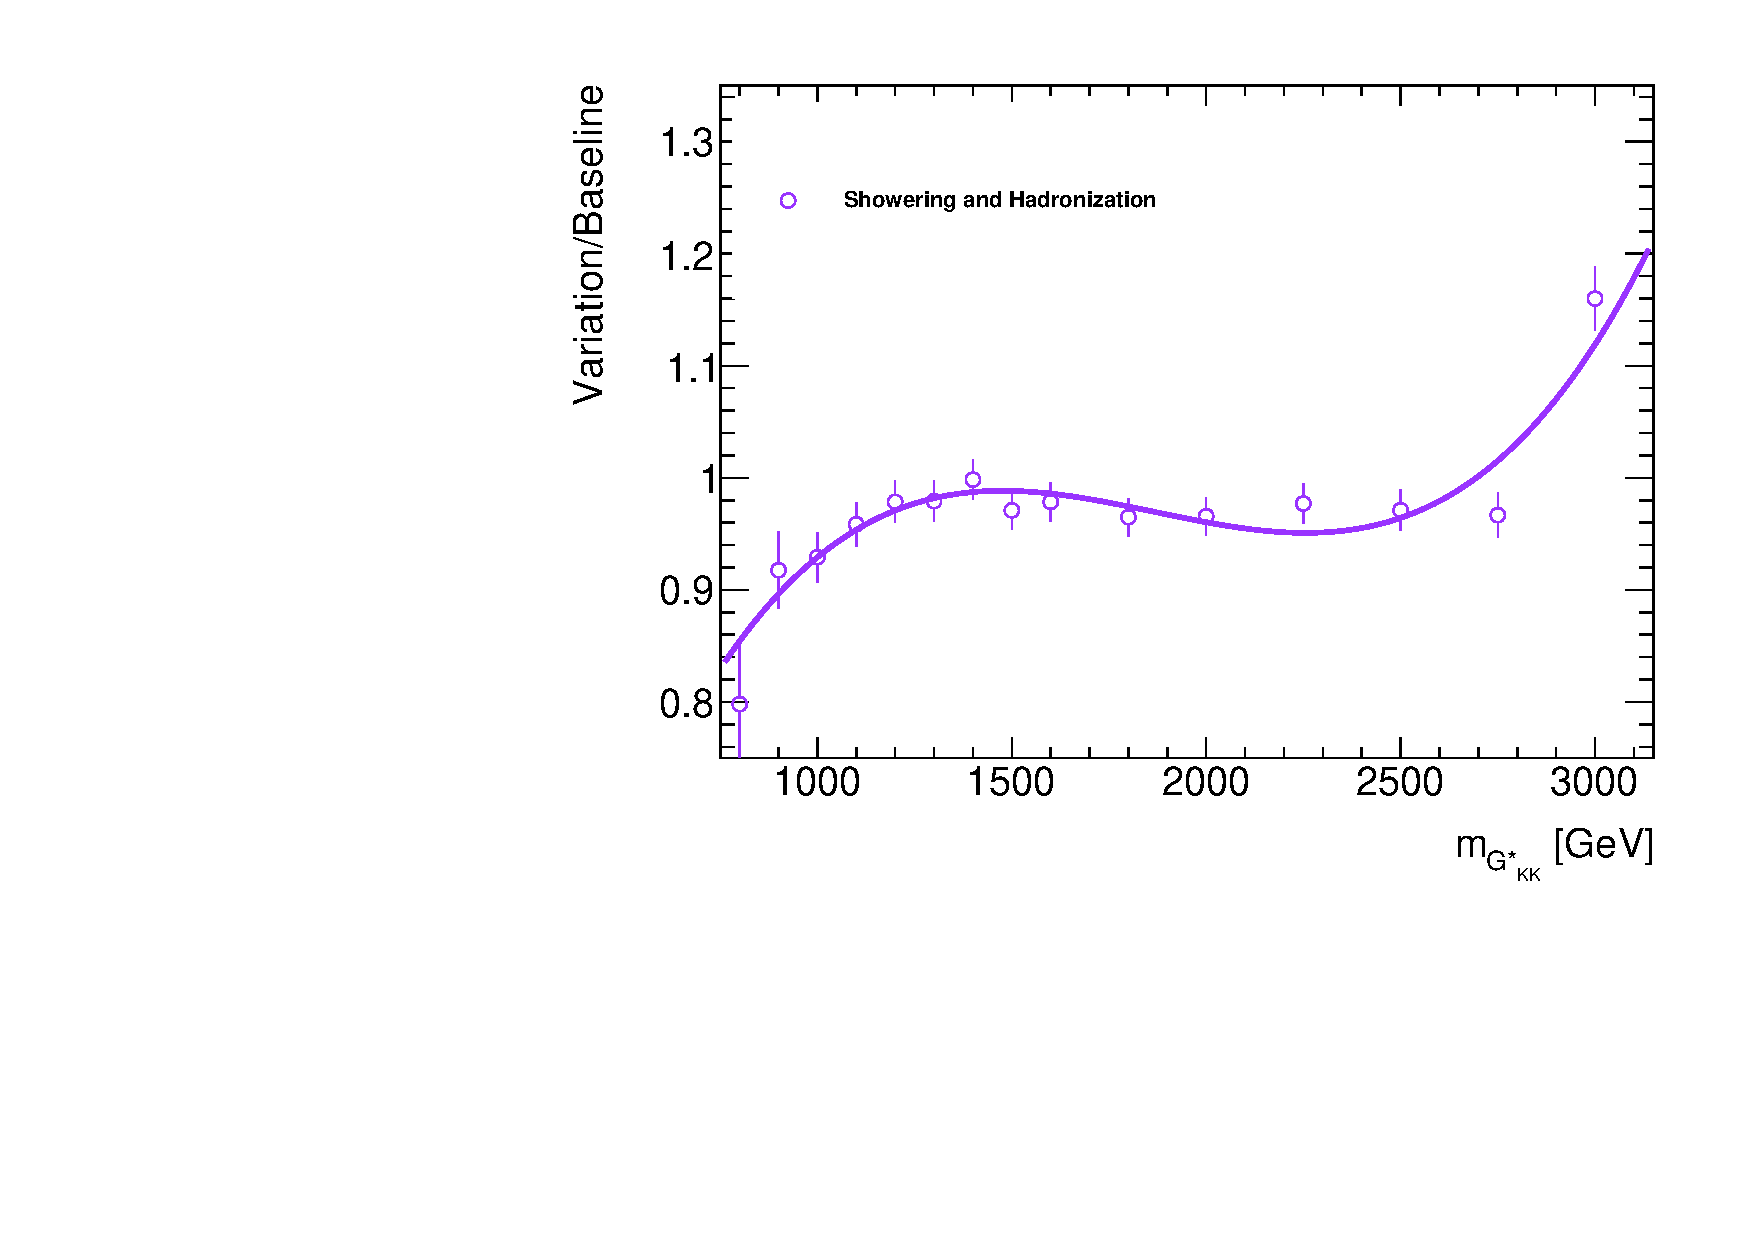
\includegraphics[width=0.3\textwidth, clip]{figures/boosted/Syst_MC/Boosted_3Tag_BulkRSGKKc1_Shower_ratio.pdf}\hspace{5mm}}
% \subfloat[3-Tag: bulk RS c=2]{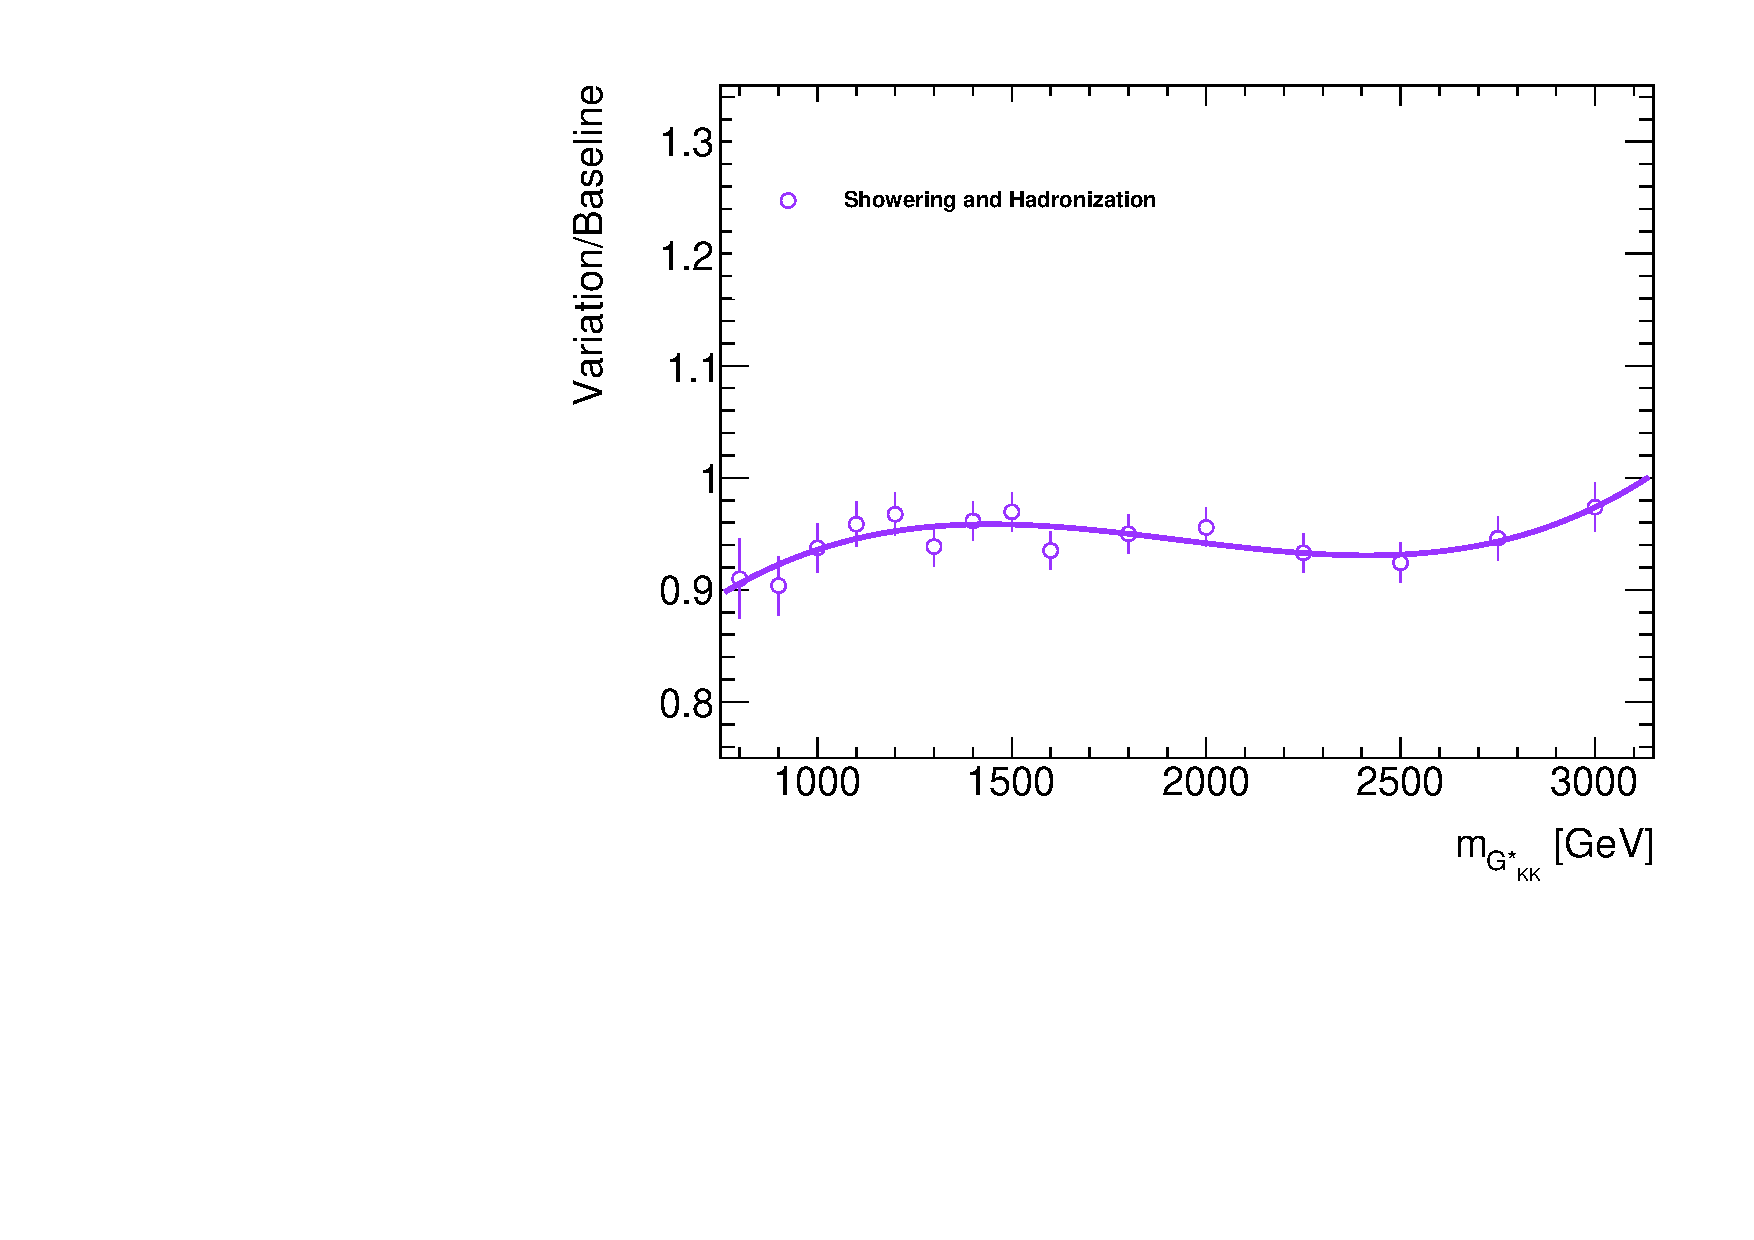
\includegraphics[width=0.3\textwidth, clip]{figures/boosted/Syst_MC/Boosted_3Tag_BulkRSGKKc2_Shower_ratio.pdf}\hspace{5mm}}
% \subfloat[3-Tag: scalar]{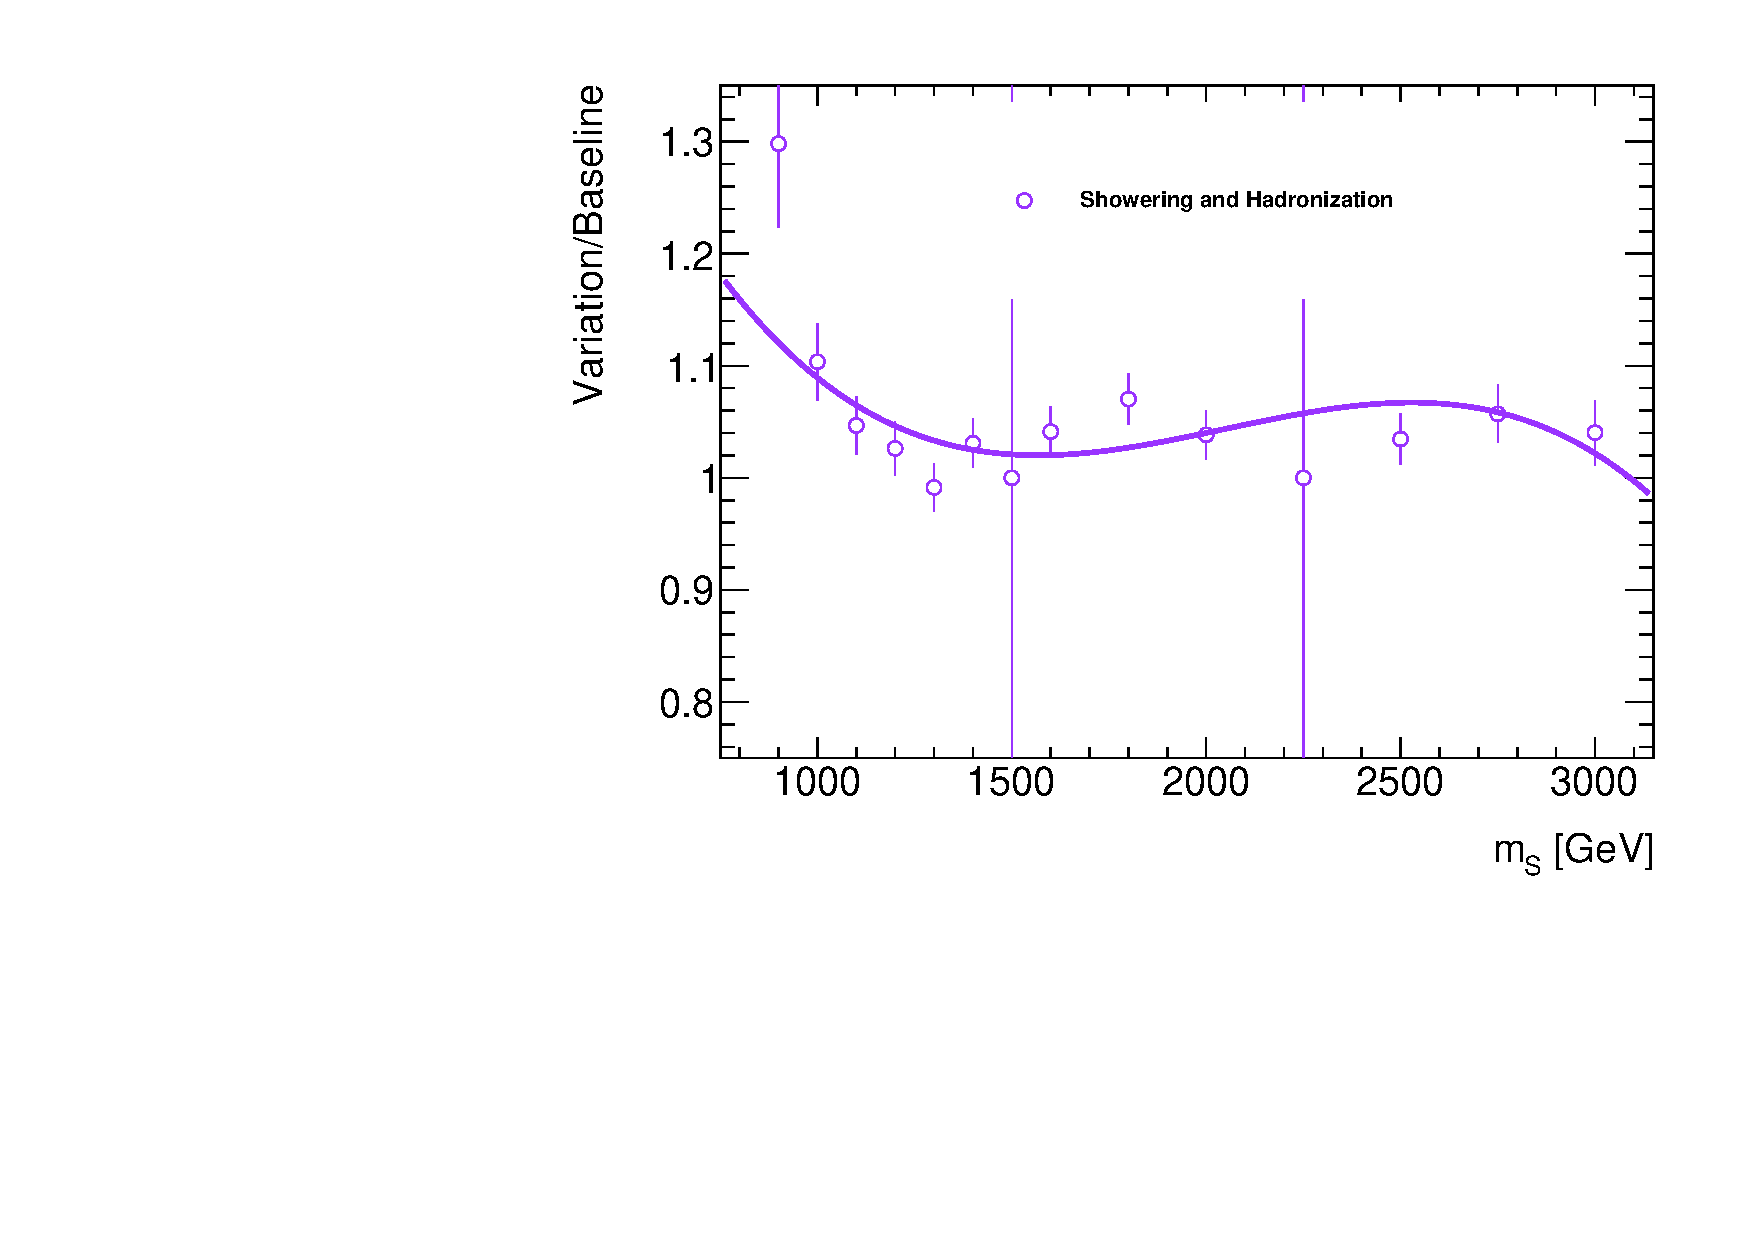
\includegraphics[width=0.3\textwidth, clip]{figures/boosted/Syst_MC/Boosted_3Tag_Scalar_Shower_ratio.pdf}\hspace{5mm}}\\
% \subfloat[4-Tag: bulk RS c=1]{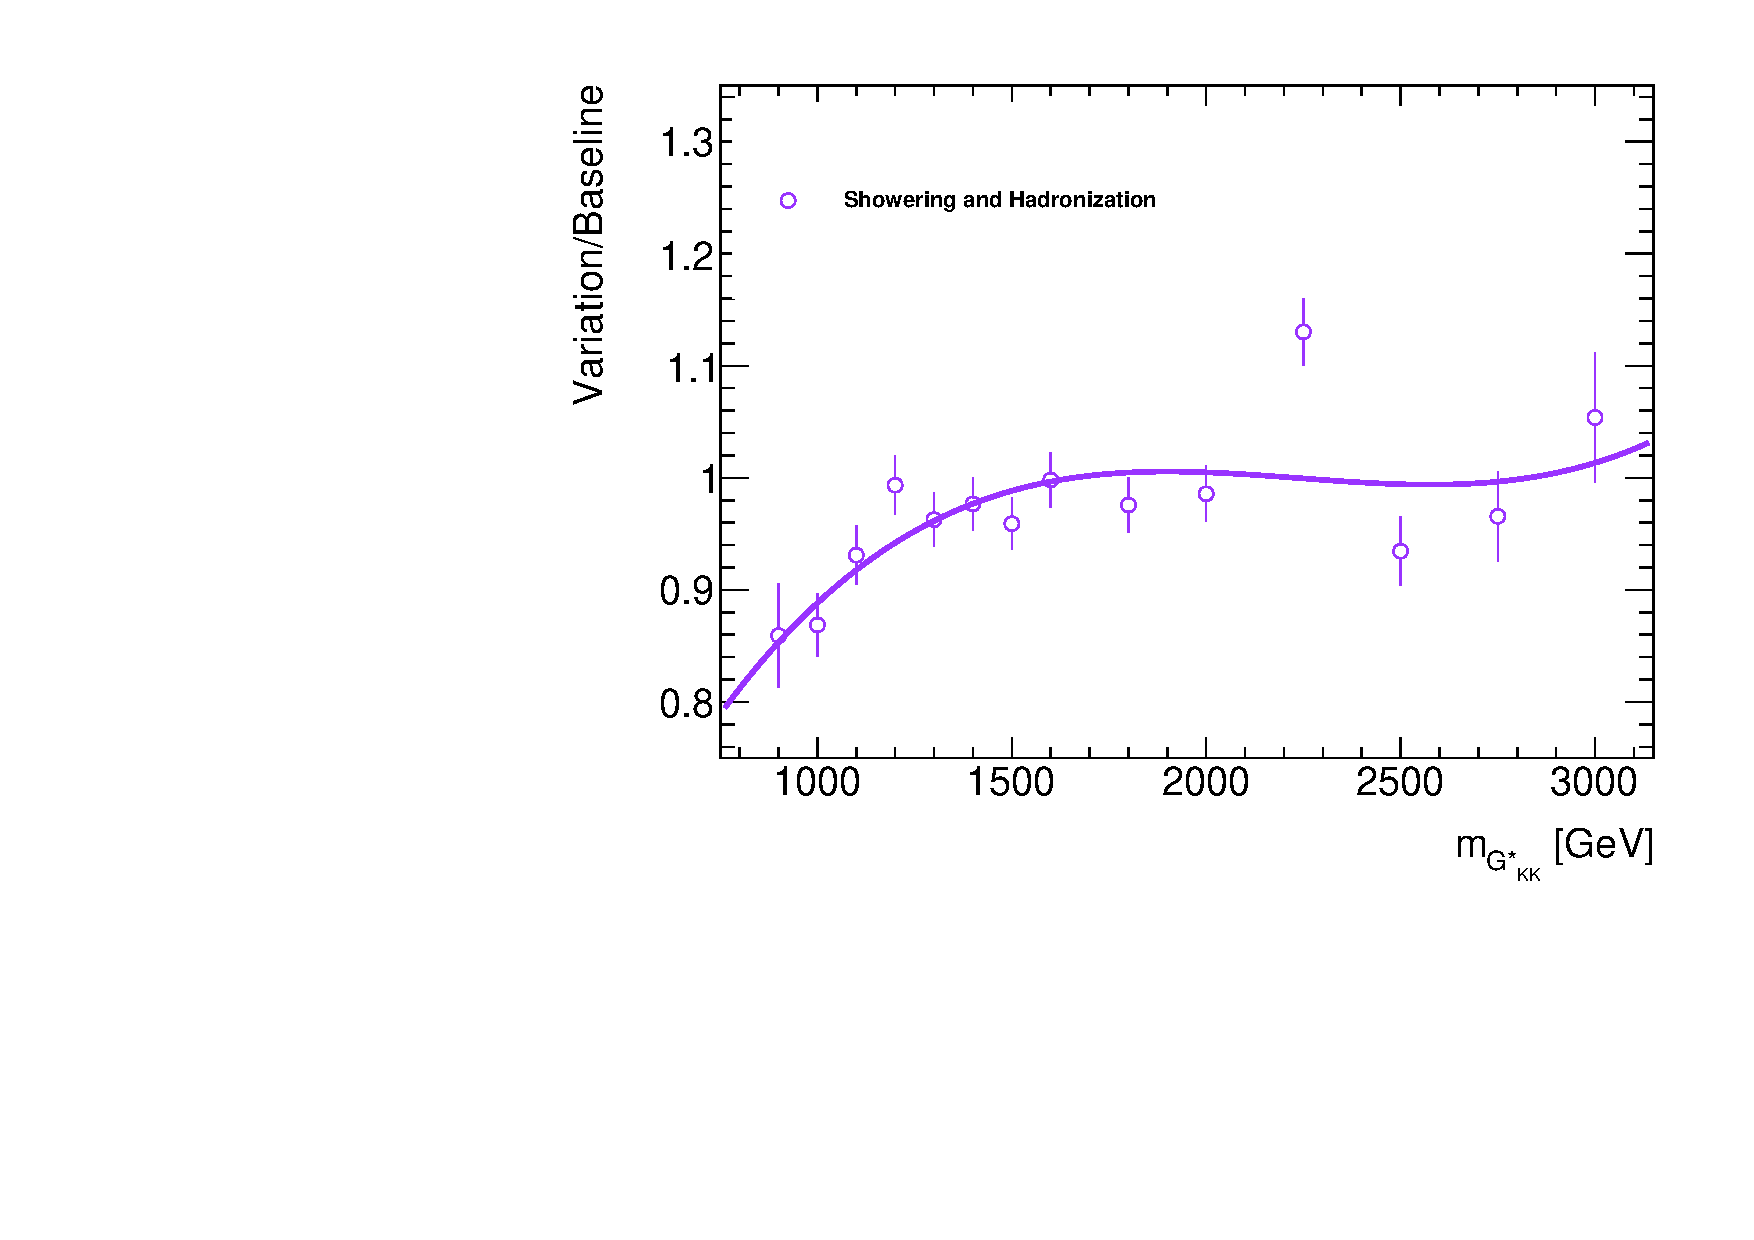
\includegraphics[width=0.3\textwidth, clip]{figures/boosted/Syst_MC/Boosted_4Tag_BulkRSGKKc1_Shower_ratio.pdf}\hspace{5mm}}
% \subfloat[4-Tag: bulk RS c=2]{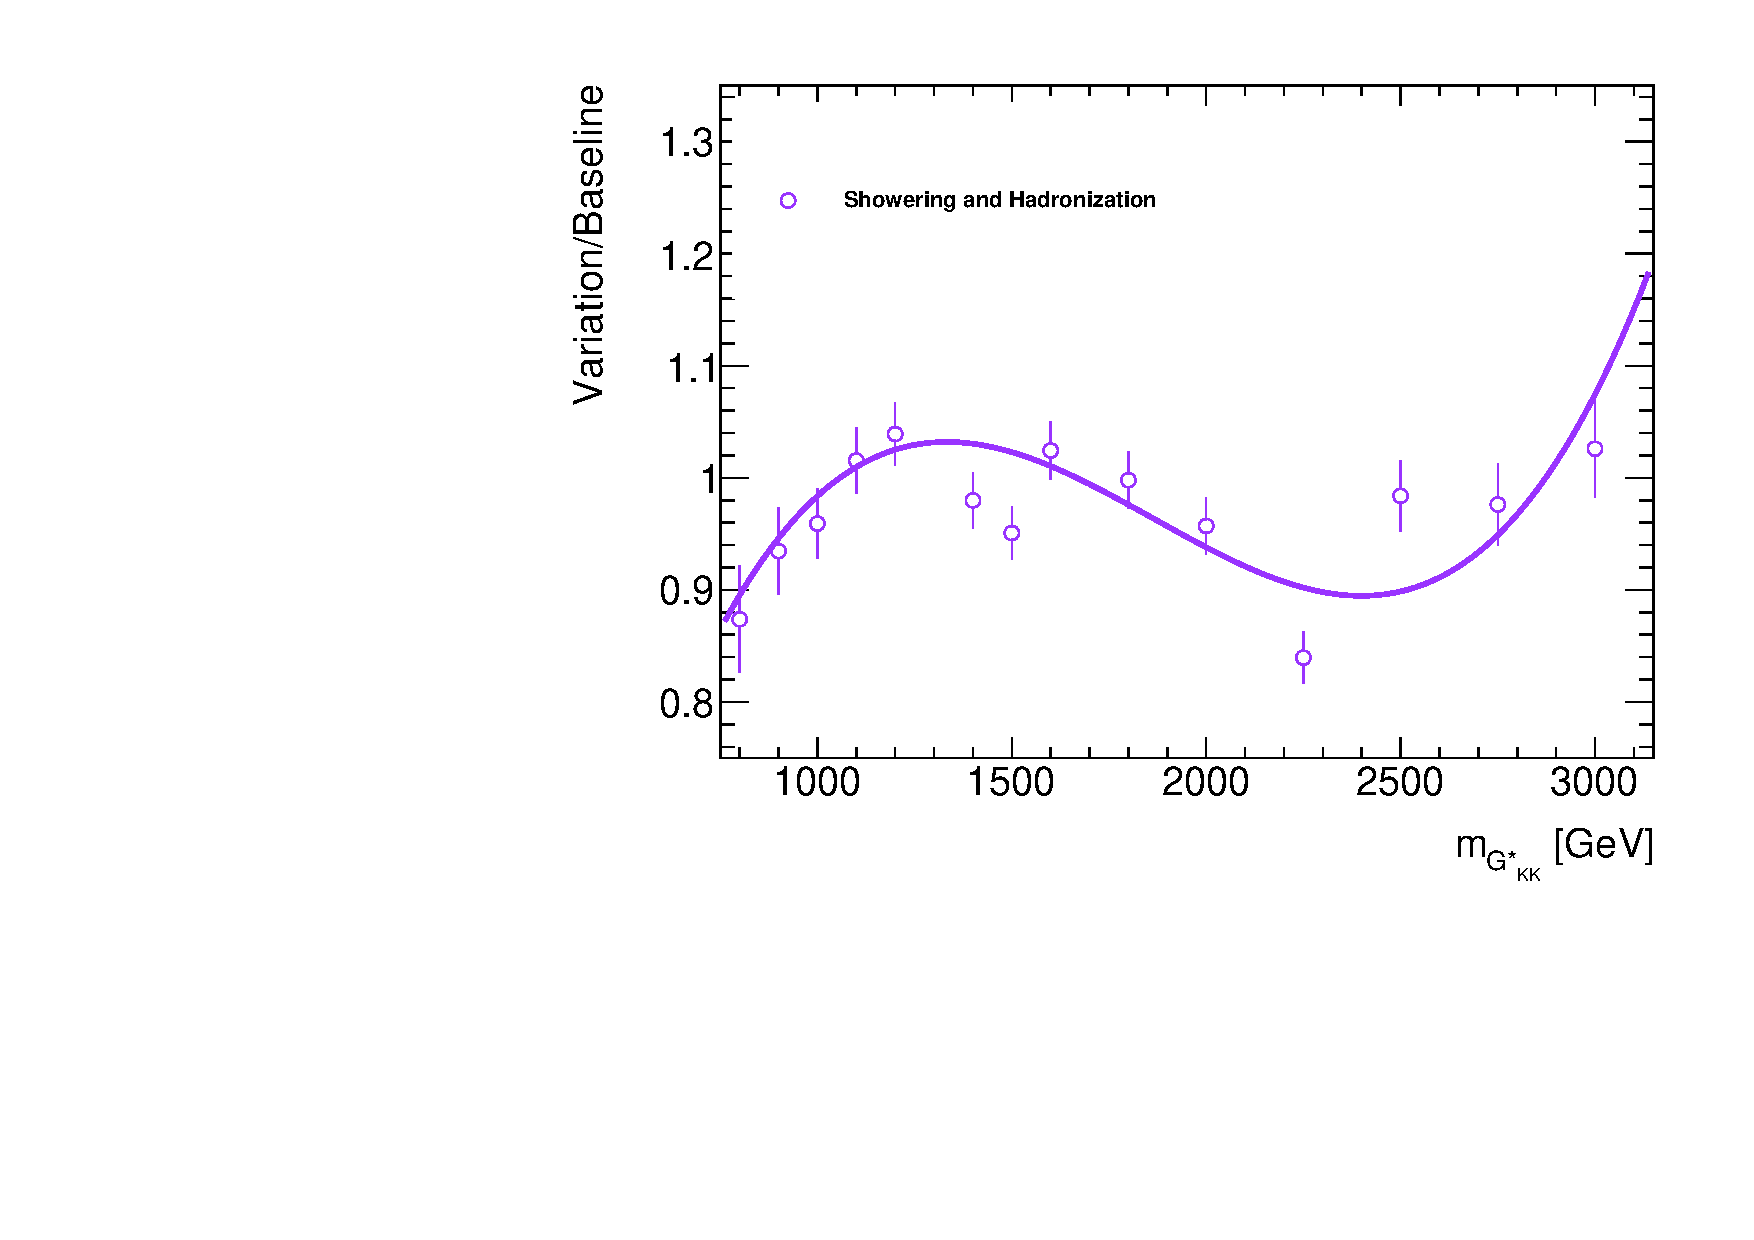
\includegraphics[width=0.3\textwidth, clip]{figures/boosted/Syst_MC/Boosted_4Tag_BulkRSGKKc2_Shower_ratio.pdf}\hspace{5mm}}
% \subfloat[4-Tag: scalar]{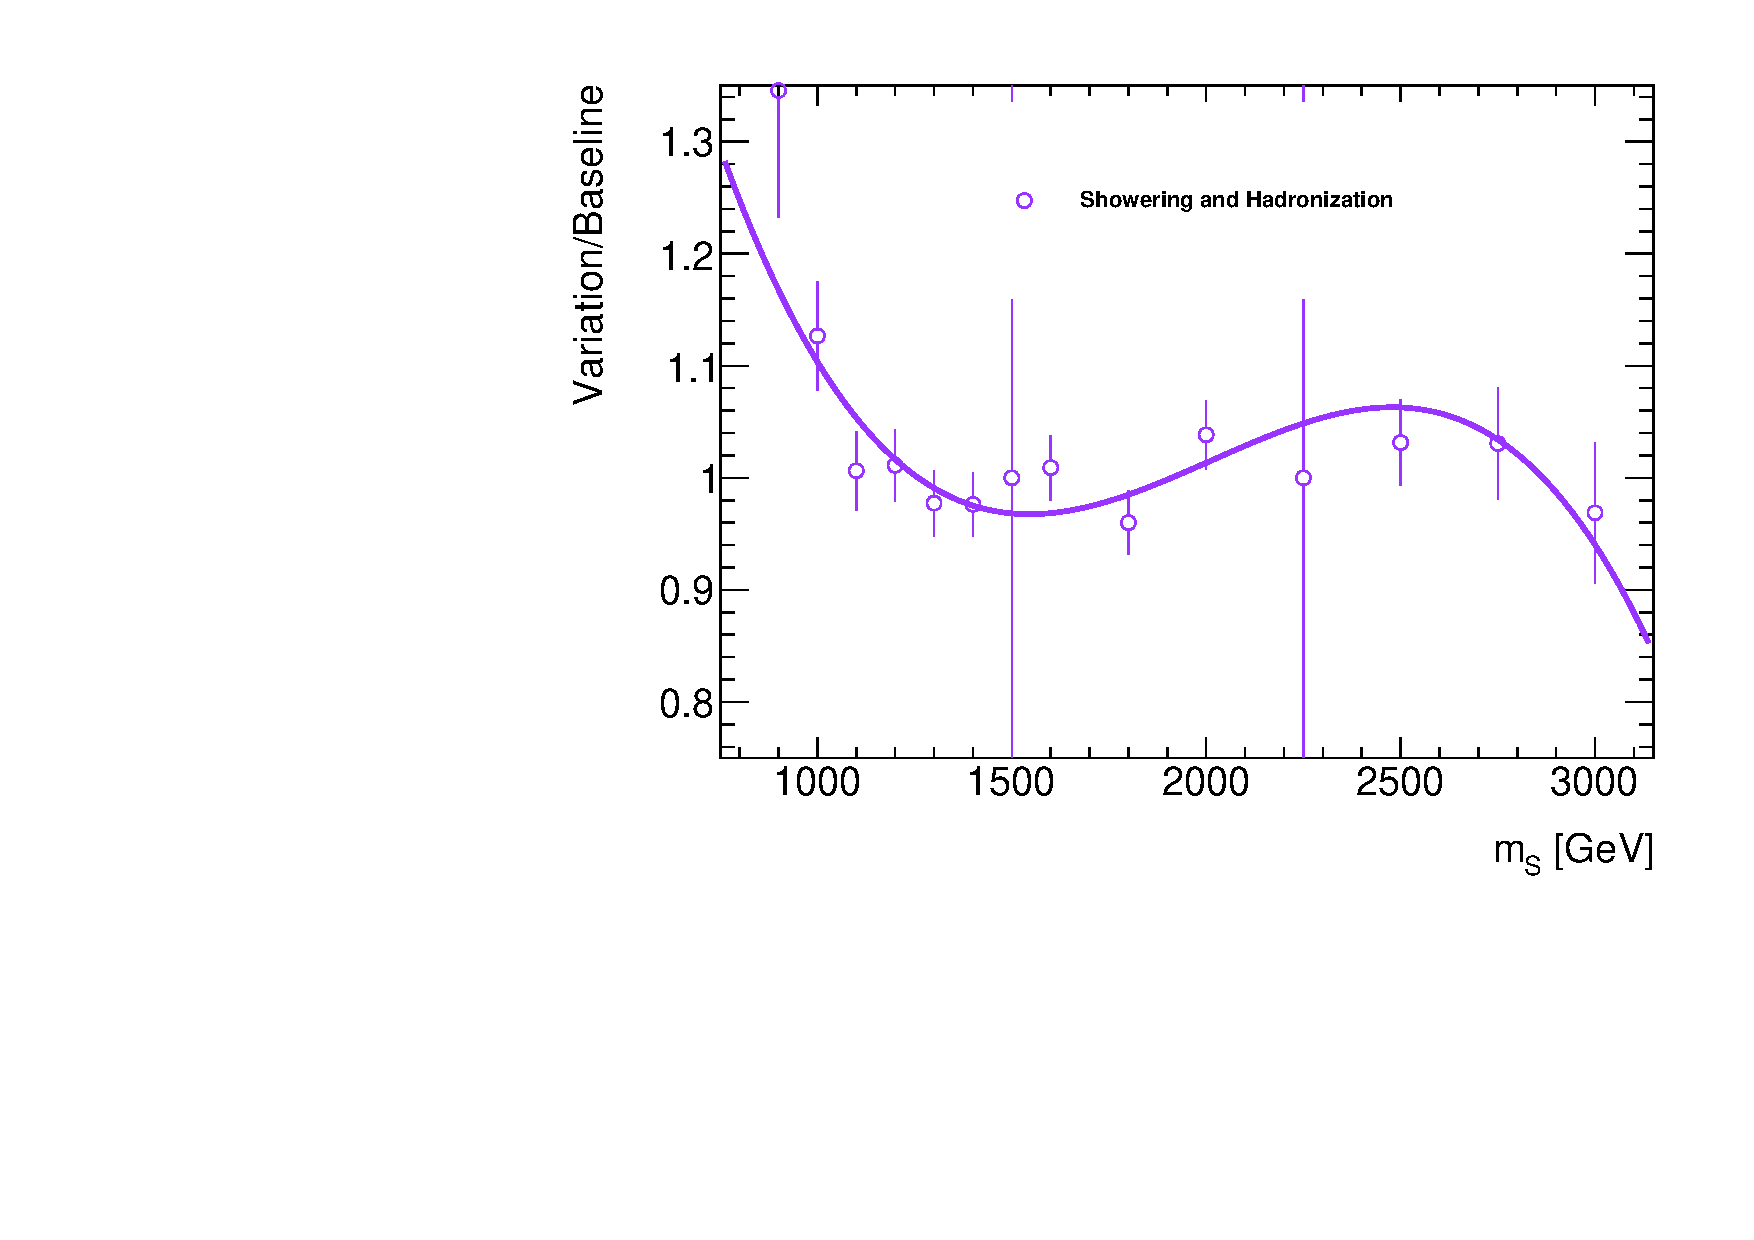
\includegraphics[width=0.3\textwidth, clip]{figures/boosted/Syst_MC/Boosted_4Tag_Scalar_Shower_ratio.pdf}\hspace{5mm}}
% \caption{Ratio of acceptance times efficiency measured in the shower-varied samples over the baseline sample shown as open circles. The polynomial fits shown as solid lines are used to assign the corresponding systematic variation in the final statistical analysis.}
% \label{fig:showerVar}
% \end{center}
% \end{figure*}

%%\paragraph{}
PDF uncertainties are evaluated using the PDF4LHC15\_nlo\_mc set, which combines CT14, MMHT14 and NNPDF3.0 PDF sets \cite{0954-3899-43-2-023001}. The uncertainty is evaluated by calculating the acceptance for each PDF replica. The standard deviation of these acceptance values divided by the baseline acceptance is taken as the PDF uncertainty. For each mass point the distribution of these ratio is compatible with a Gaussian centred on one. The calculated PDF uncertainty is shown in Figure \ref{fig:pdfVar} as upward and downward shifts from unity. The uncertainty in acceptance due to PDF uncertainties is less than $\pm1\%$ across the full mass range considered for the analysis. For this reason, it is neglected in the statistical analysis described in Section \ref{sec:statistical-analysis}.

% \begin{figure*}
% \begin{center}
% \subfloat[2-Tag-Split: bulk RS c=1]{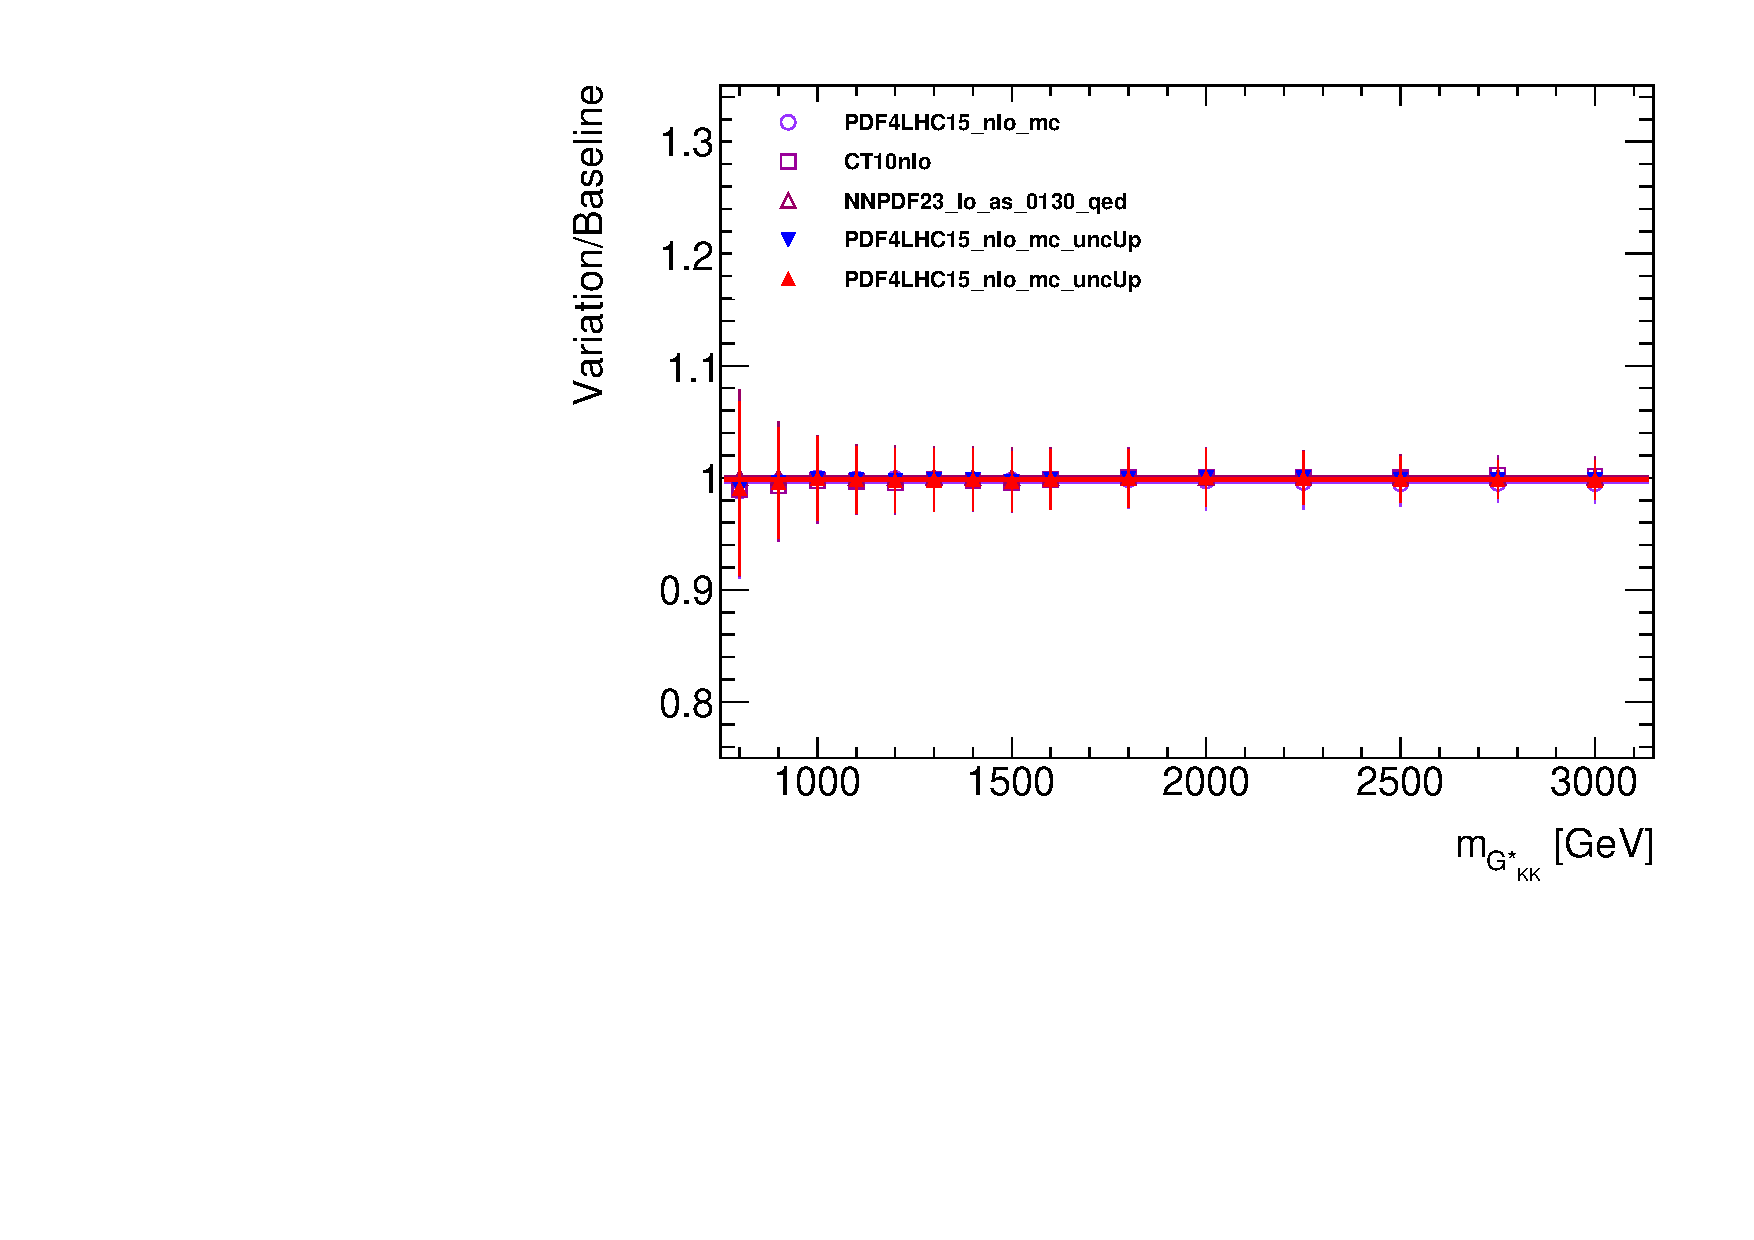
\includegraphics[width=0.3\textwidth, clip]{figures/boosted/Syst_MC/Boosted_2Tag_BulkRSGKKc1_PDF_ratio.pdf}\hspace{5mm}}
% \subfloat[2-Tag-Split: bulk RS c=2]{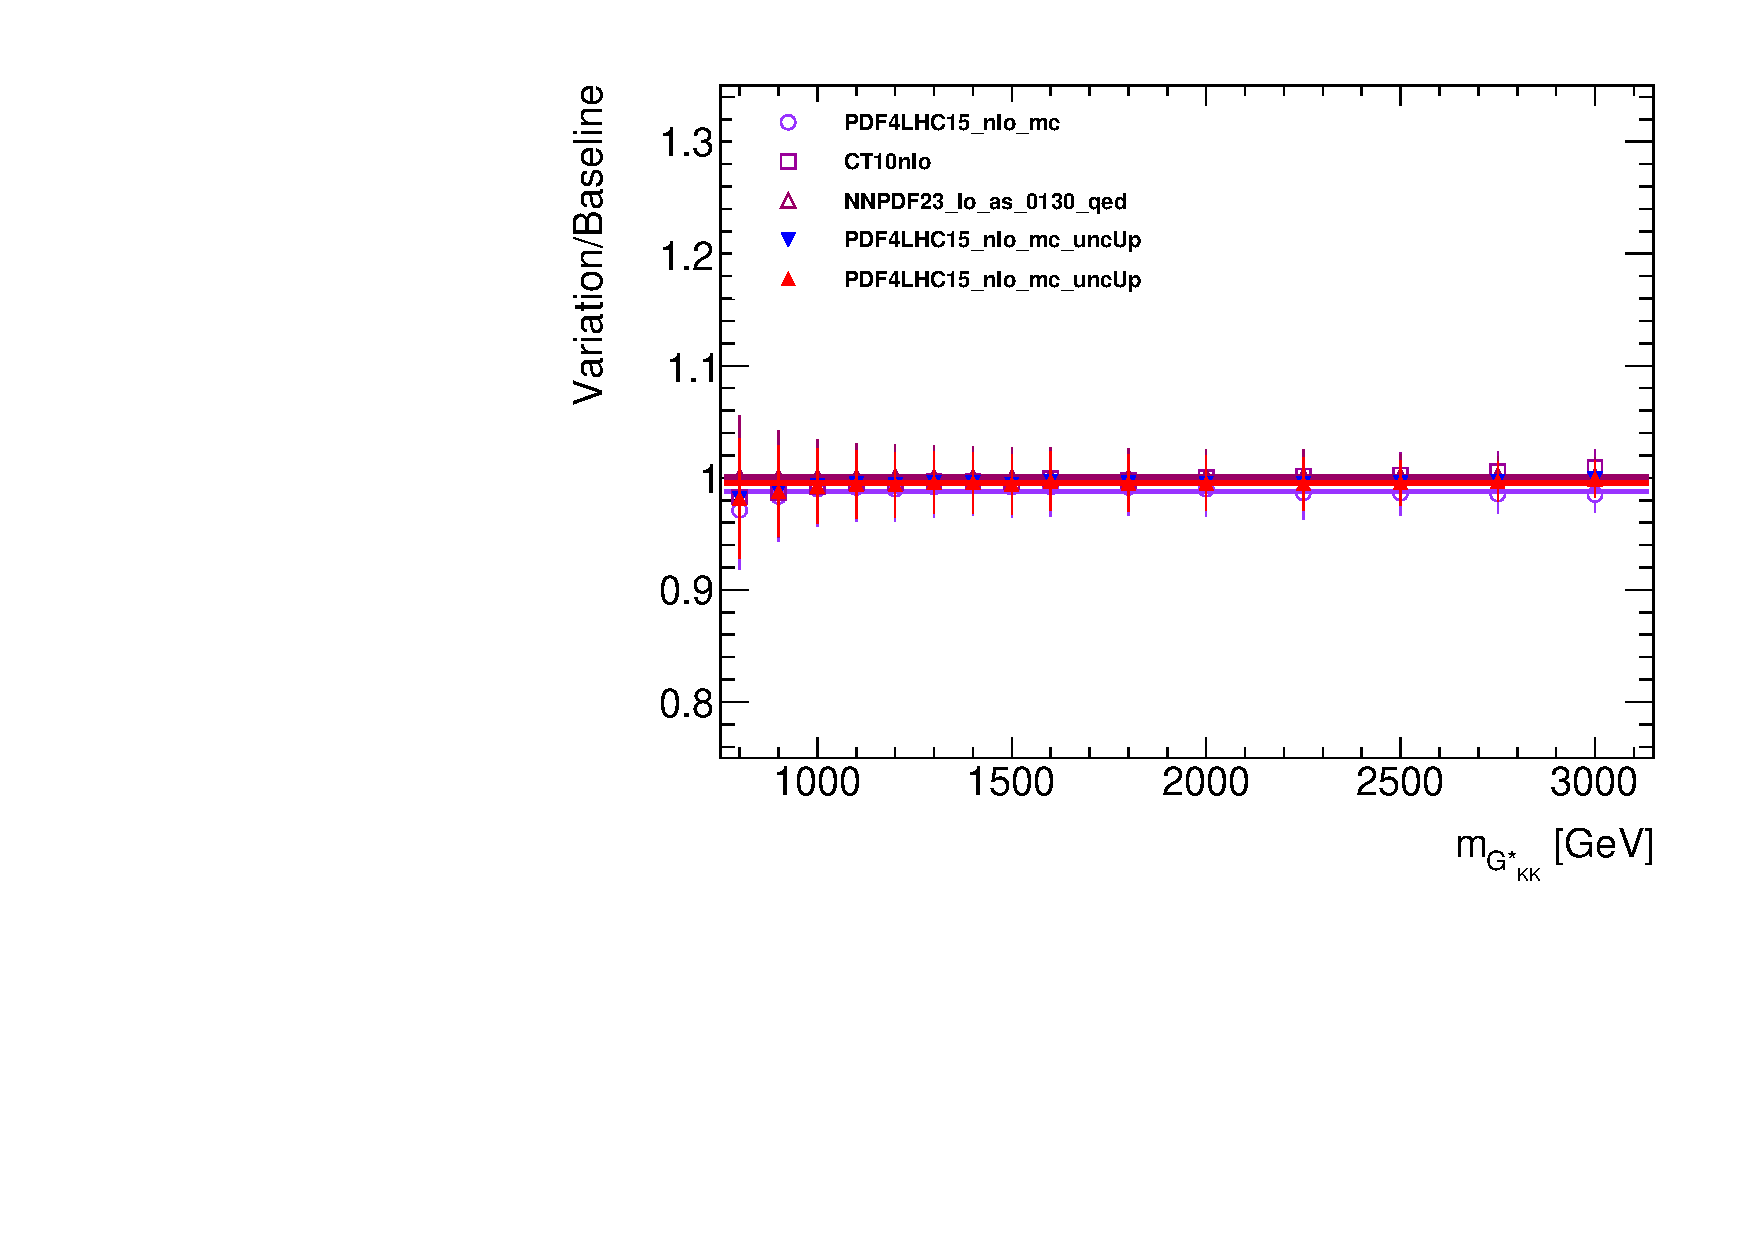
\includegraphics[width=0.3\textwidth, clip]{figures/boosted/Syst_MC/Boosted_2Tag_BulkRSGKKc2_PDF_ratio.pdf}\hspace{5mm}}
% \subfloat[2-Tag-Split: scalar]{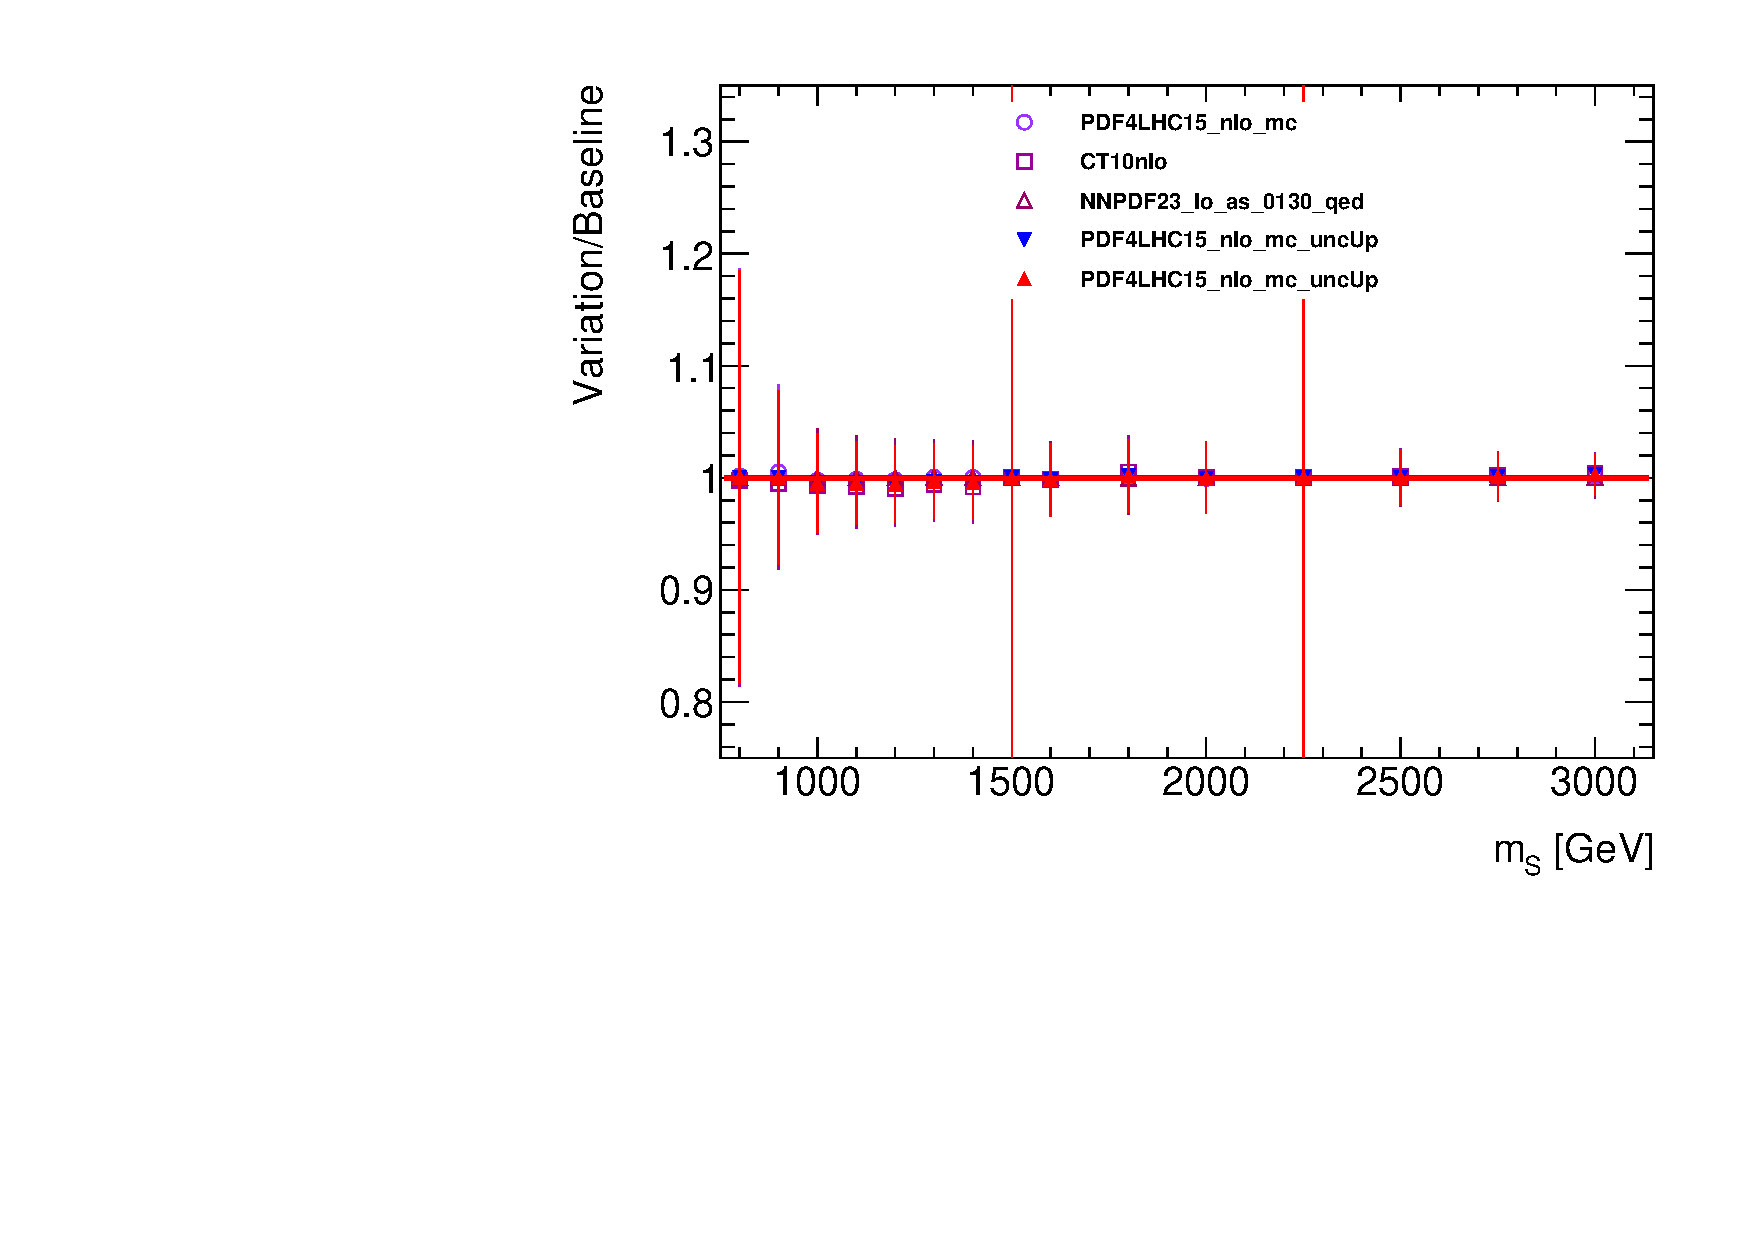
\includegraphics[width=0.3\textwidth, clip]{figures/boosted/Syst_MC/Boosted_2Tag_Scalar_PDF_ratio.pdf}\hspace{5mm}}\\
% \subfloat[3-Tag: bulk RS c=1]{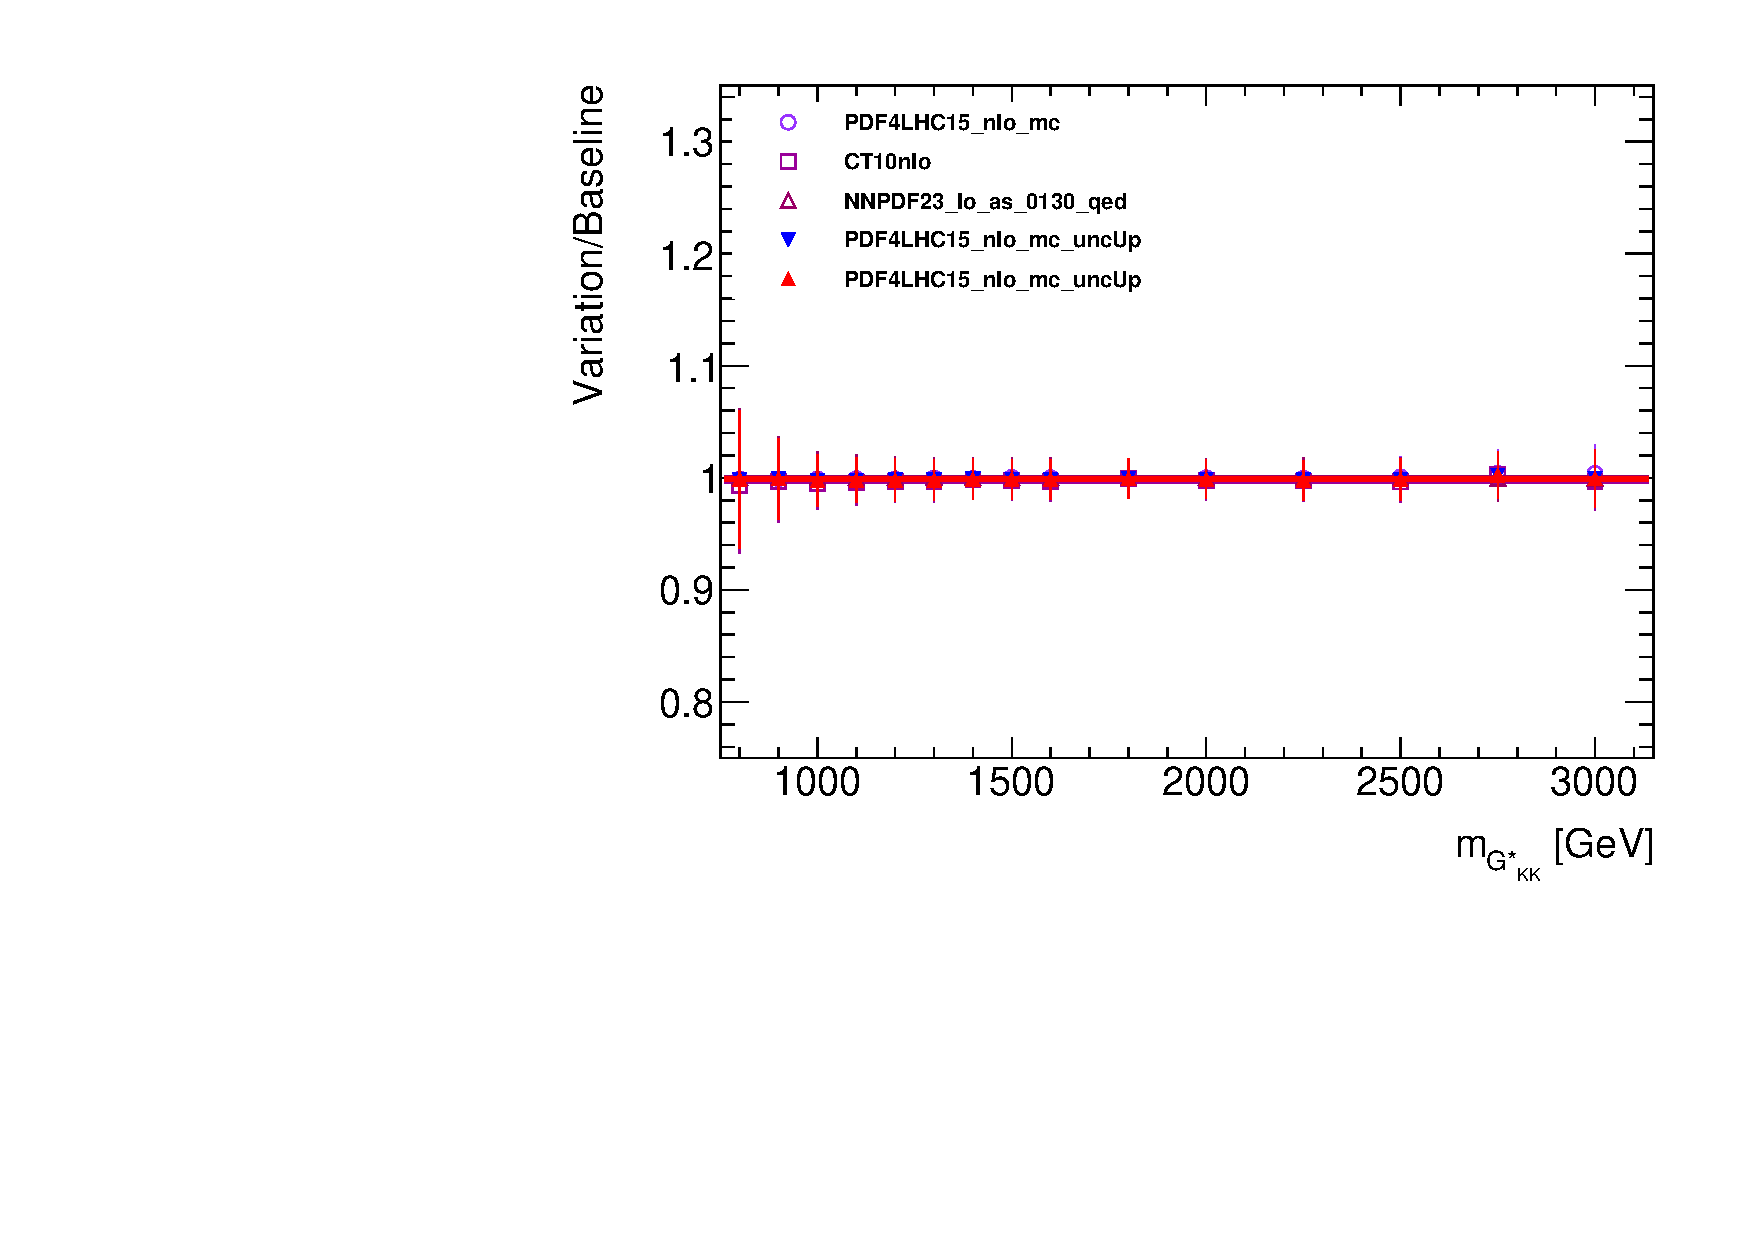
\includegraphics[width=0.3\textwidth, clip]{figures/boosted/Syst_MC/Boosted_3Tag_BulkRSGKKc1_PDF_ratio.pdf}\hspace{5mm}}
% \subfloat[3-Tag: bulk RS c=2]{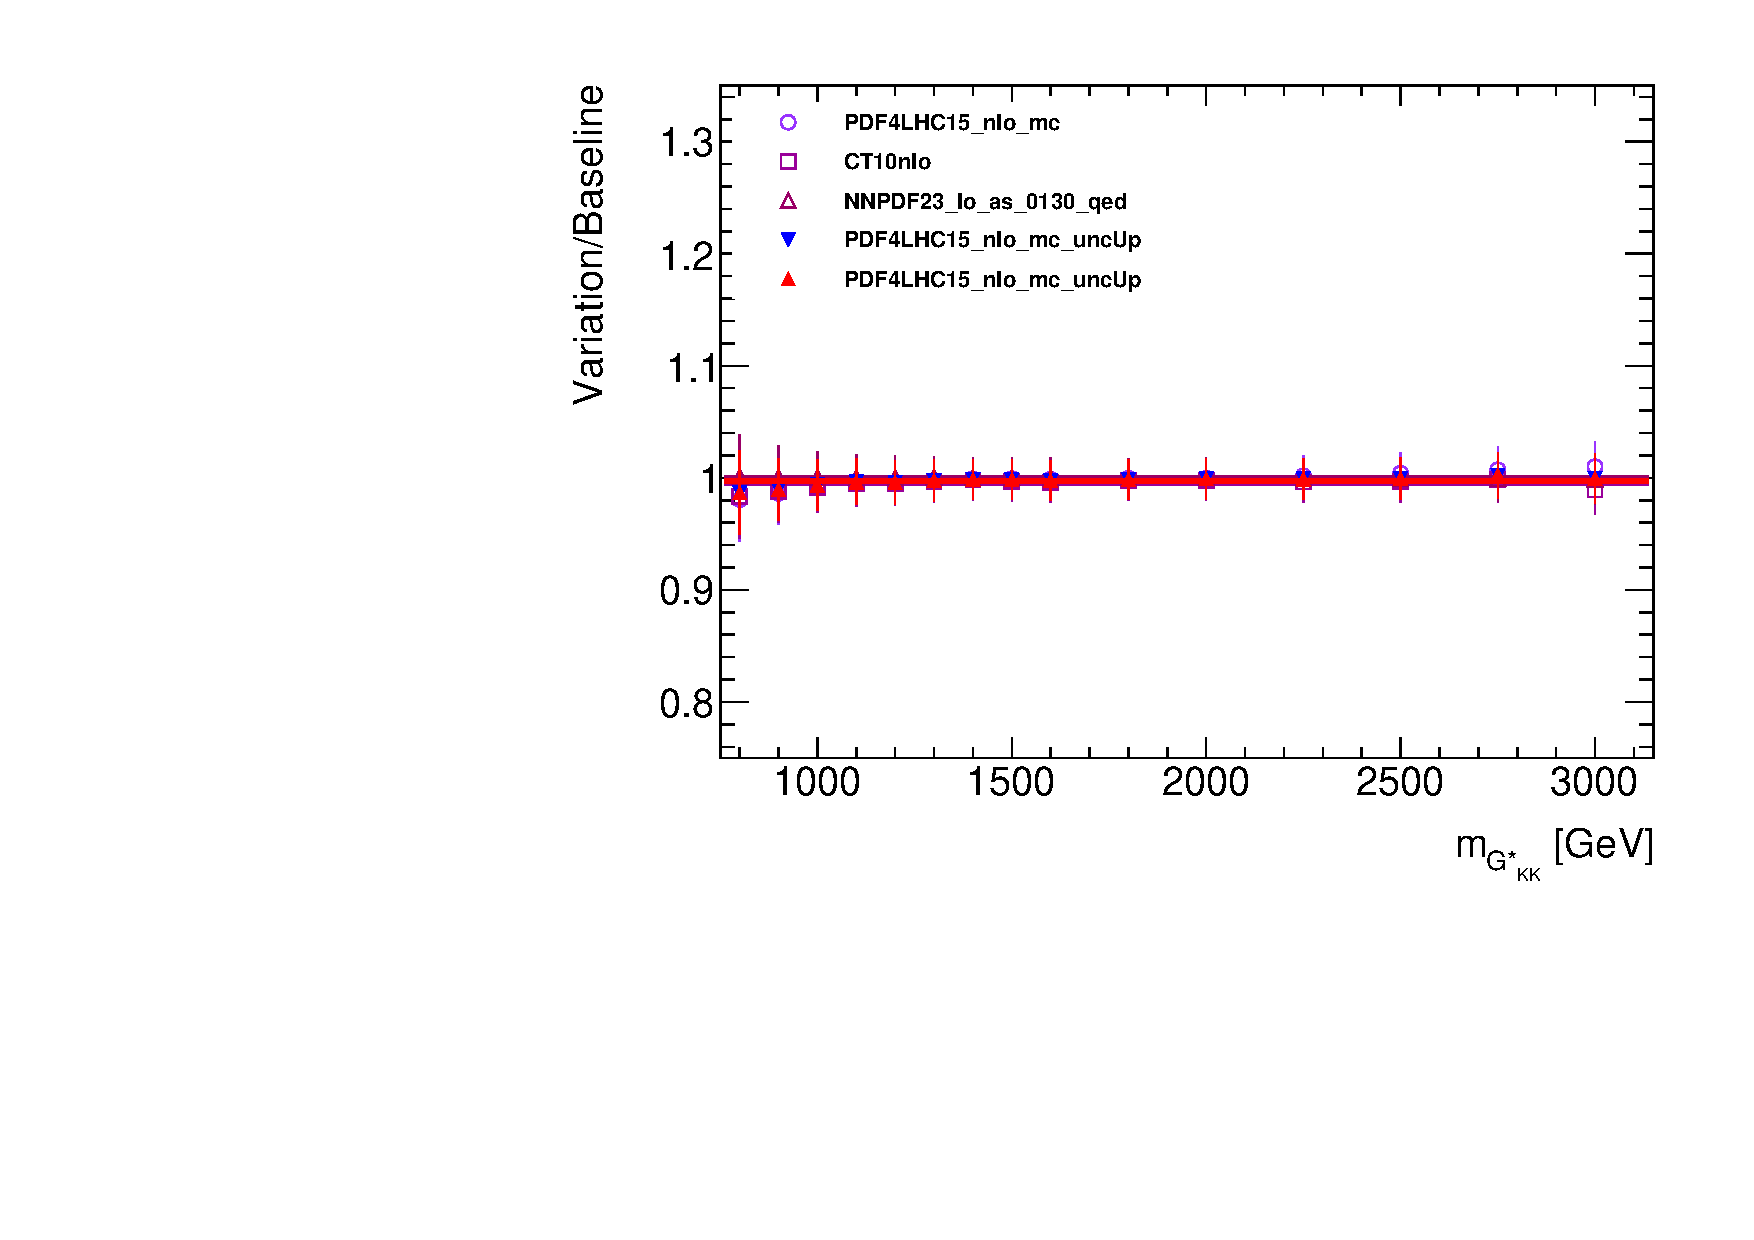
\includegraphics[width=0.3\textwidth, clip]{figures/boosted/Syst_MC/Boosted_3Tag_BulkRSGKKc2_PDF_ratio.pdf}\hspace{5mm}}
% \subfloat[3-Tag: scalar]{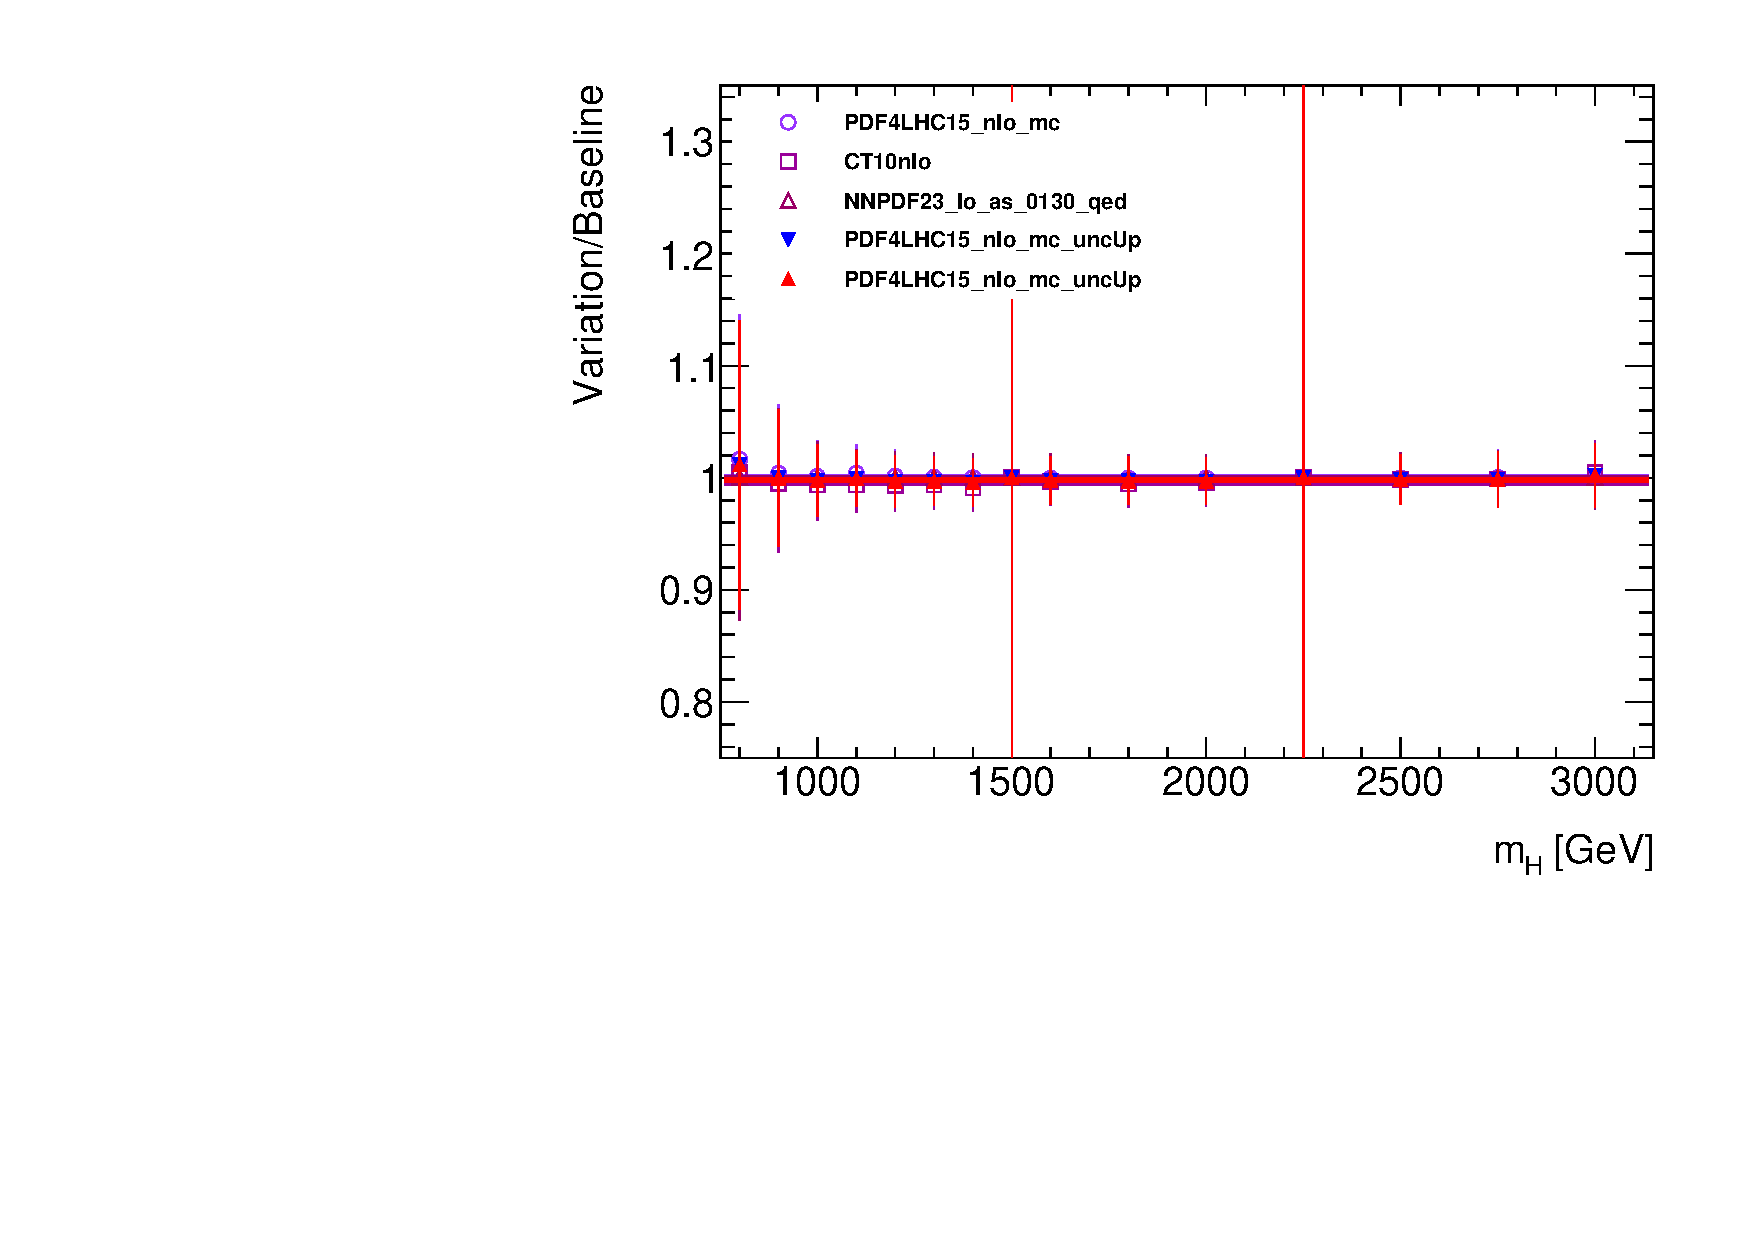
\includegraphics[width=0.3\textwidth, clip]{figures/boosted/Syst_MC/Boosted_3Tag_Scalar_PDF_ratio.pdf}\hspace{5mm}}\\
% \subfloat[4-Tag: bulk RS c=1]{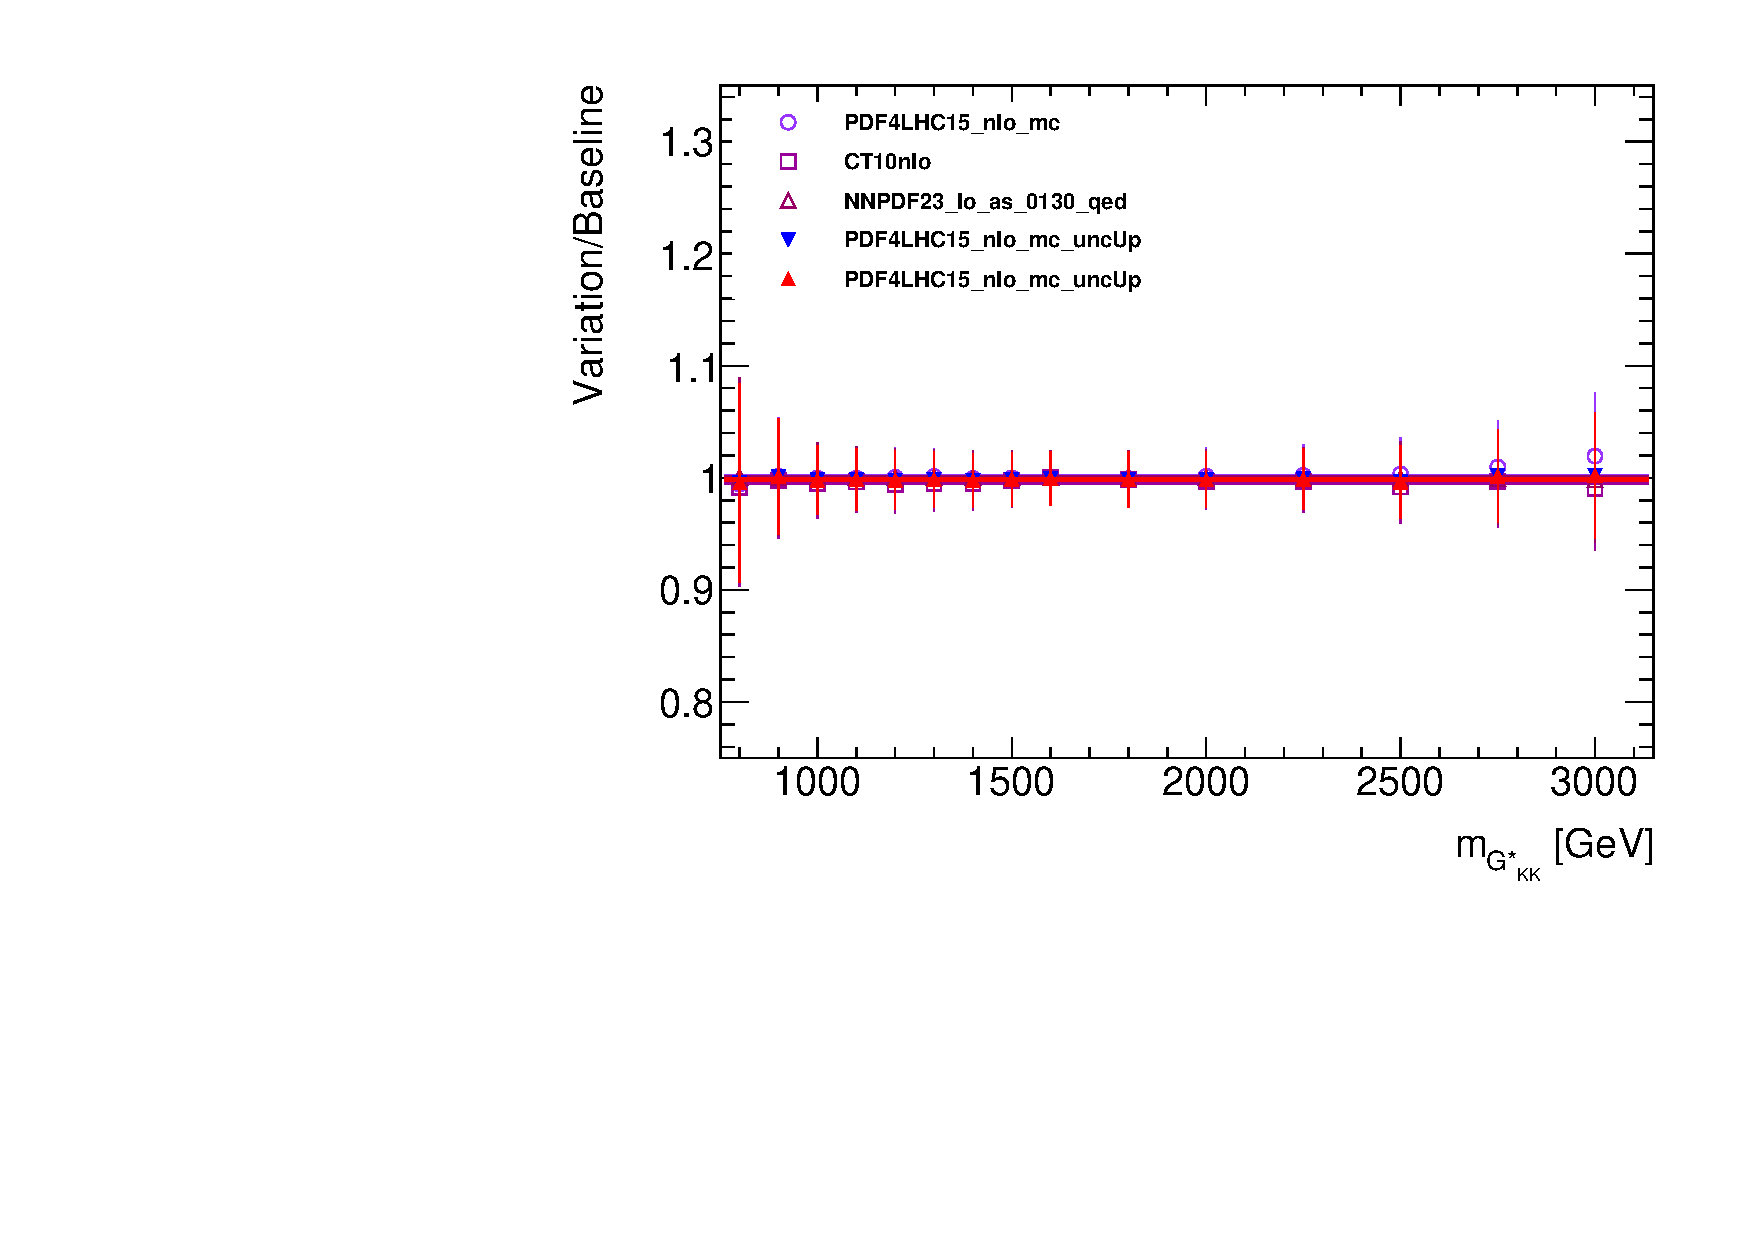
\includegraphics[width=0.3\textwidth, clip]{figures/boosted/Syst_MC/Boosted_4Tag_BulkRSGKKc1_PDF_ratio.pdf}\hspace{5mm}}
% \subfloat[4-Tag: bulk RS c=2]{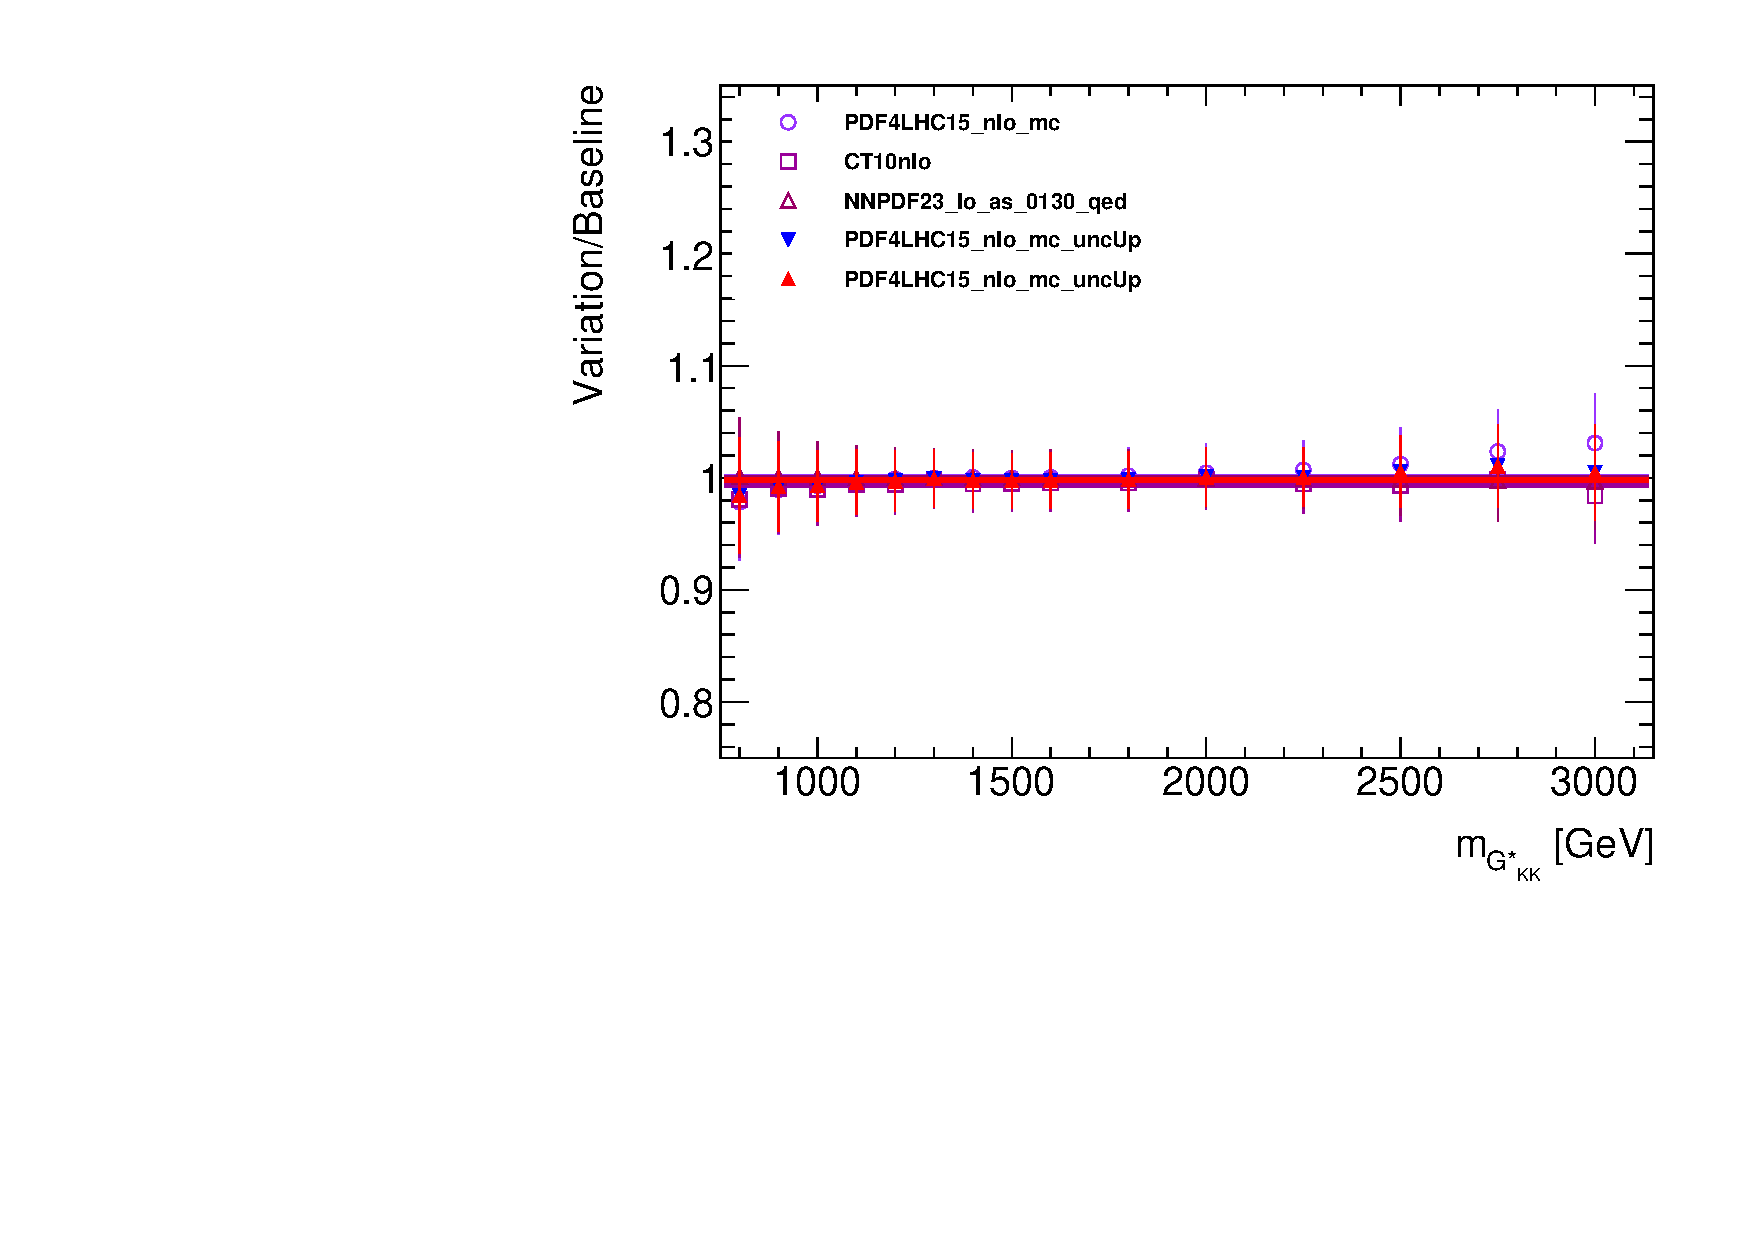
\includegraphics[width=0.3\textwidth, clip]{figures/boosted/Syst_MC/Boosted_4Tag_BulkRSGKKc2_PDF_ratio.pdf}\hspace{5mm}}
% \subfloat[4-Tag: scalar]{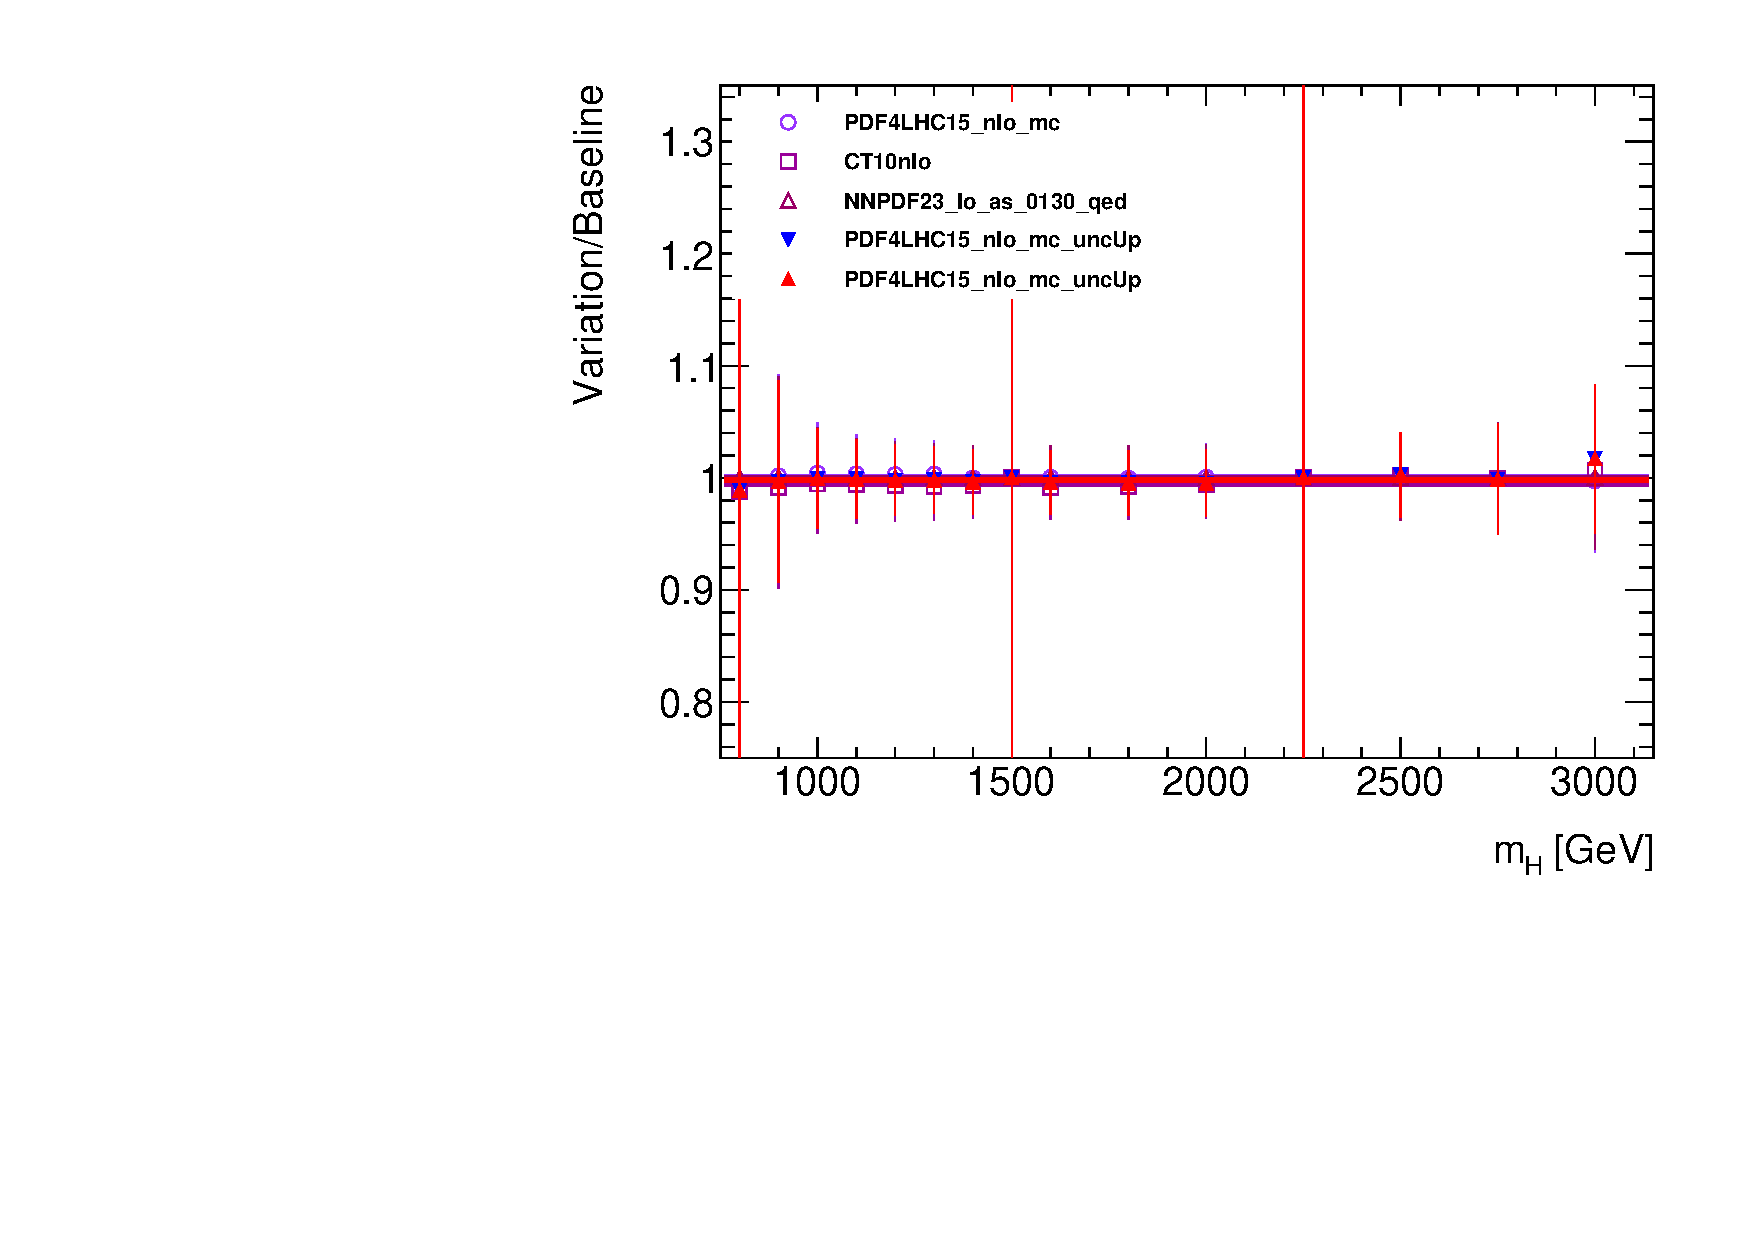
\includegraphics[width=0.3\textwidth, clip]{figures/boosted/Syst_MC/Boosted_4Tag_Scalar_PDF_ratio.pdf}\hspace{5mm}}
% \caption{Ratio of acceptance times efficiency measured in the PDF-varied samples over the baseline sample shown as open circles. Given the consistency with unity, no PDF-uncertainty will be assigned.}
% \label{fig:pdfVar}
% \end{center}
% \end{figure*}

These uncertainties are implemented in the final statistical analysis as normalisation uncertainties on the signals, with the value taken from the polynomial fit. This smooths out statistical fluctuations and allows interpolation between the generated mass points, if needed.